\documentclass[aspectratio=169]{beamer}

% ---------------------------------------------------------------------
% DORI -- Figures, Tables & Calibration Equations (Chapters 2-4 + Appendix)
% ---------------------------------------------------------------------

\usetheme{default}
\usecolortheme{default}
\setbeamertemplate{navigation symbols}{}
\setbeamertemplate{footline}[frame number]
\setbeamercolor{background canvas}{bg=white}
\setbeamercolor{normal text}{fg=black}

\usepackage[utf8]{inputenc}
\usepackage[T1]{fontenc}
\usepackage[english]{babel}
\usepackage{amsmath,amssymb,bm}
\usepackage{graphicx}
\usepackage{tikz}
\usepackage{adjustbox}
\usepackage{xcolor}
\usepackage{booktabs}
\usepackage{multirow}
\usepackage{array}
\usepackage{tabularx}
\usepackage[absolute,overlay]{textpos}
\textblockorigin{0pt}{0pt}

\definecolor{doriblue}{RGB}{26,111,223}
\definecolor{dorigold}{RGB}{204,153,0}

% ---------------------------------------------------------------------
% Custom frame title: fat blue horizontal bar, white bold text.
% Placed with textpos at absolute (0,0) so it is immune to beamer's
% internal side-margin length and always spans the full slide width.
% ---------------------------------------------------------------------
\newlength{\titlebarht}
\setlength{\titlebarht}{1.35cm}
\setbeamerfont{frametitle}{series=\bfseries,size=\large}
\setbeamertemplate{frametitle}{%
  \begin{textblock*}{\paperwidth}(0pt,0pt)
    \colorbox{doriblue}{%
      \makebox[\paperwidth][l]{\hspace{0.5cm}%
        \parbox[c][\titlebarht][c]{\dimexpr\paperwidth-1cm\relax}{%
          \usebeamerfont{frametitle}\color{white}\insertframetitle}}%
    }
  \end{textblock*}
  \vspace{\titlebarht}\vspace{2mm}%
}

% Section divider: full blue slide, white title
\newcommand{\sectiondivider}[1]{%
  \begingroup
  \setbeamercolor{background canvas}{bg=doriblue}
  \begin{frame}[plain]
    \vfill
    \centering
    {\usebeamerfont{frametitle}\bfseries\color{white}\Huge #1}
    \vfill
  \end{frame}
  \endgroup
}

\newcommand{\smallcap}[1]{{\footnotesize\color{black!70} #1\par}}

\title{DORI: Hardware, Calibration \& Final Prototype}
\subtitle{Every figure, table and calibration equation --- Chapters 2 to 4 and Appendix}
\author{Marta Alexandra Moniz Rodrigues}
\date{\today}

\begin{document}

% ======================================================================
\begin{frame}[plain]
  \centering
  \vspace{1cm}
  {\Huge\bfseries\color{doriblue} DORI}\\[0.3cm]
  {\Large Hardware, Calibration \& Final Prototype}\\[0.15cm]
  {\large\color{black!60} Every figure, table and calibration equation --- Chapters 2--4 and Appendix}\\[1.2cm]
  {\large Marta Alexandra Moniz Rodrigues}\\[0.2cm]
  {\normalsize\today}
\end{frame}

% ======================================================================
\begin{frame}
  \frametitle{Contents}
  \begin{columns}[T]
    \begin{column}{0.5\textwidth}
      \begin{itemize}
        \item[\color{doriblue}\textbullet] Ch.~2 --- Hardware Development
        \item[\color{doriblue}\textbullet] Ch.~3 --- Calibration of the DORI Prototype
      \end{itemize}
    \end{column}
    \begin{column}{0.5\textwidth}
      \begin{itemize}
        \item[\color{doriblue}\textbullet] Ch.~4 --- Final Prototype
        \item[\color{doriblue}\textbullet] Appendix
      \end{itemize}
    \end{column}
  \end{columns}
\end{frame}

% ======================================================================
\sectiondivider{Chapter 2\\[4pt]\Large Hardware Development}

% ---- fig:DORI ---------------------------------------------------------
\begin{frame}
  \frametitle{Conceptual Design of DORI}
  \begin{center}
    \adjustbox{max width=0.62\textwidth,max height=0.6\textheight}{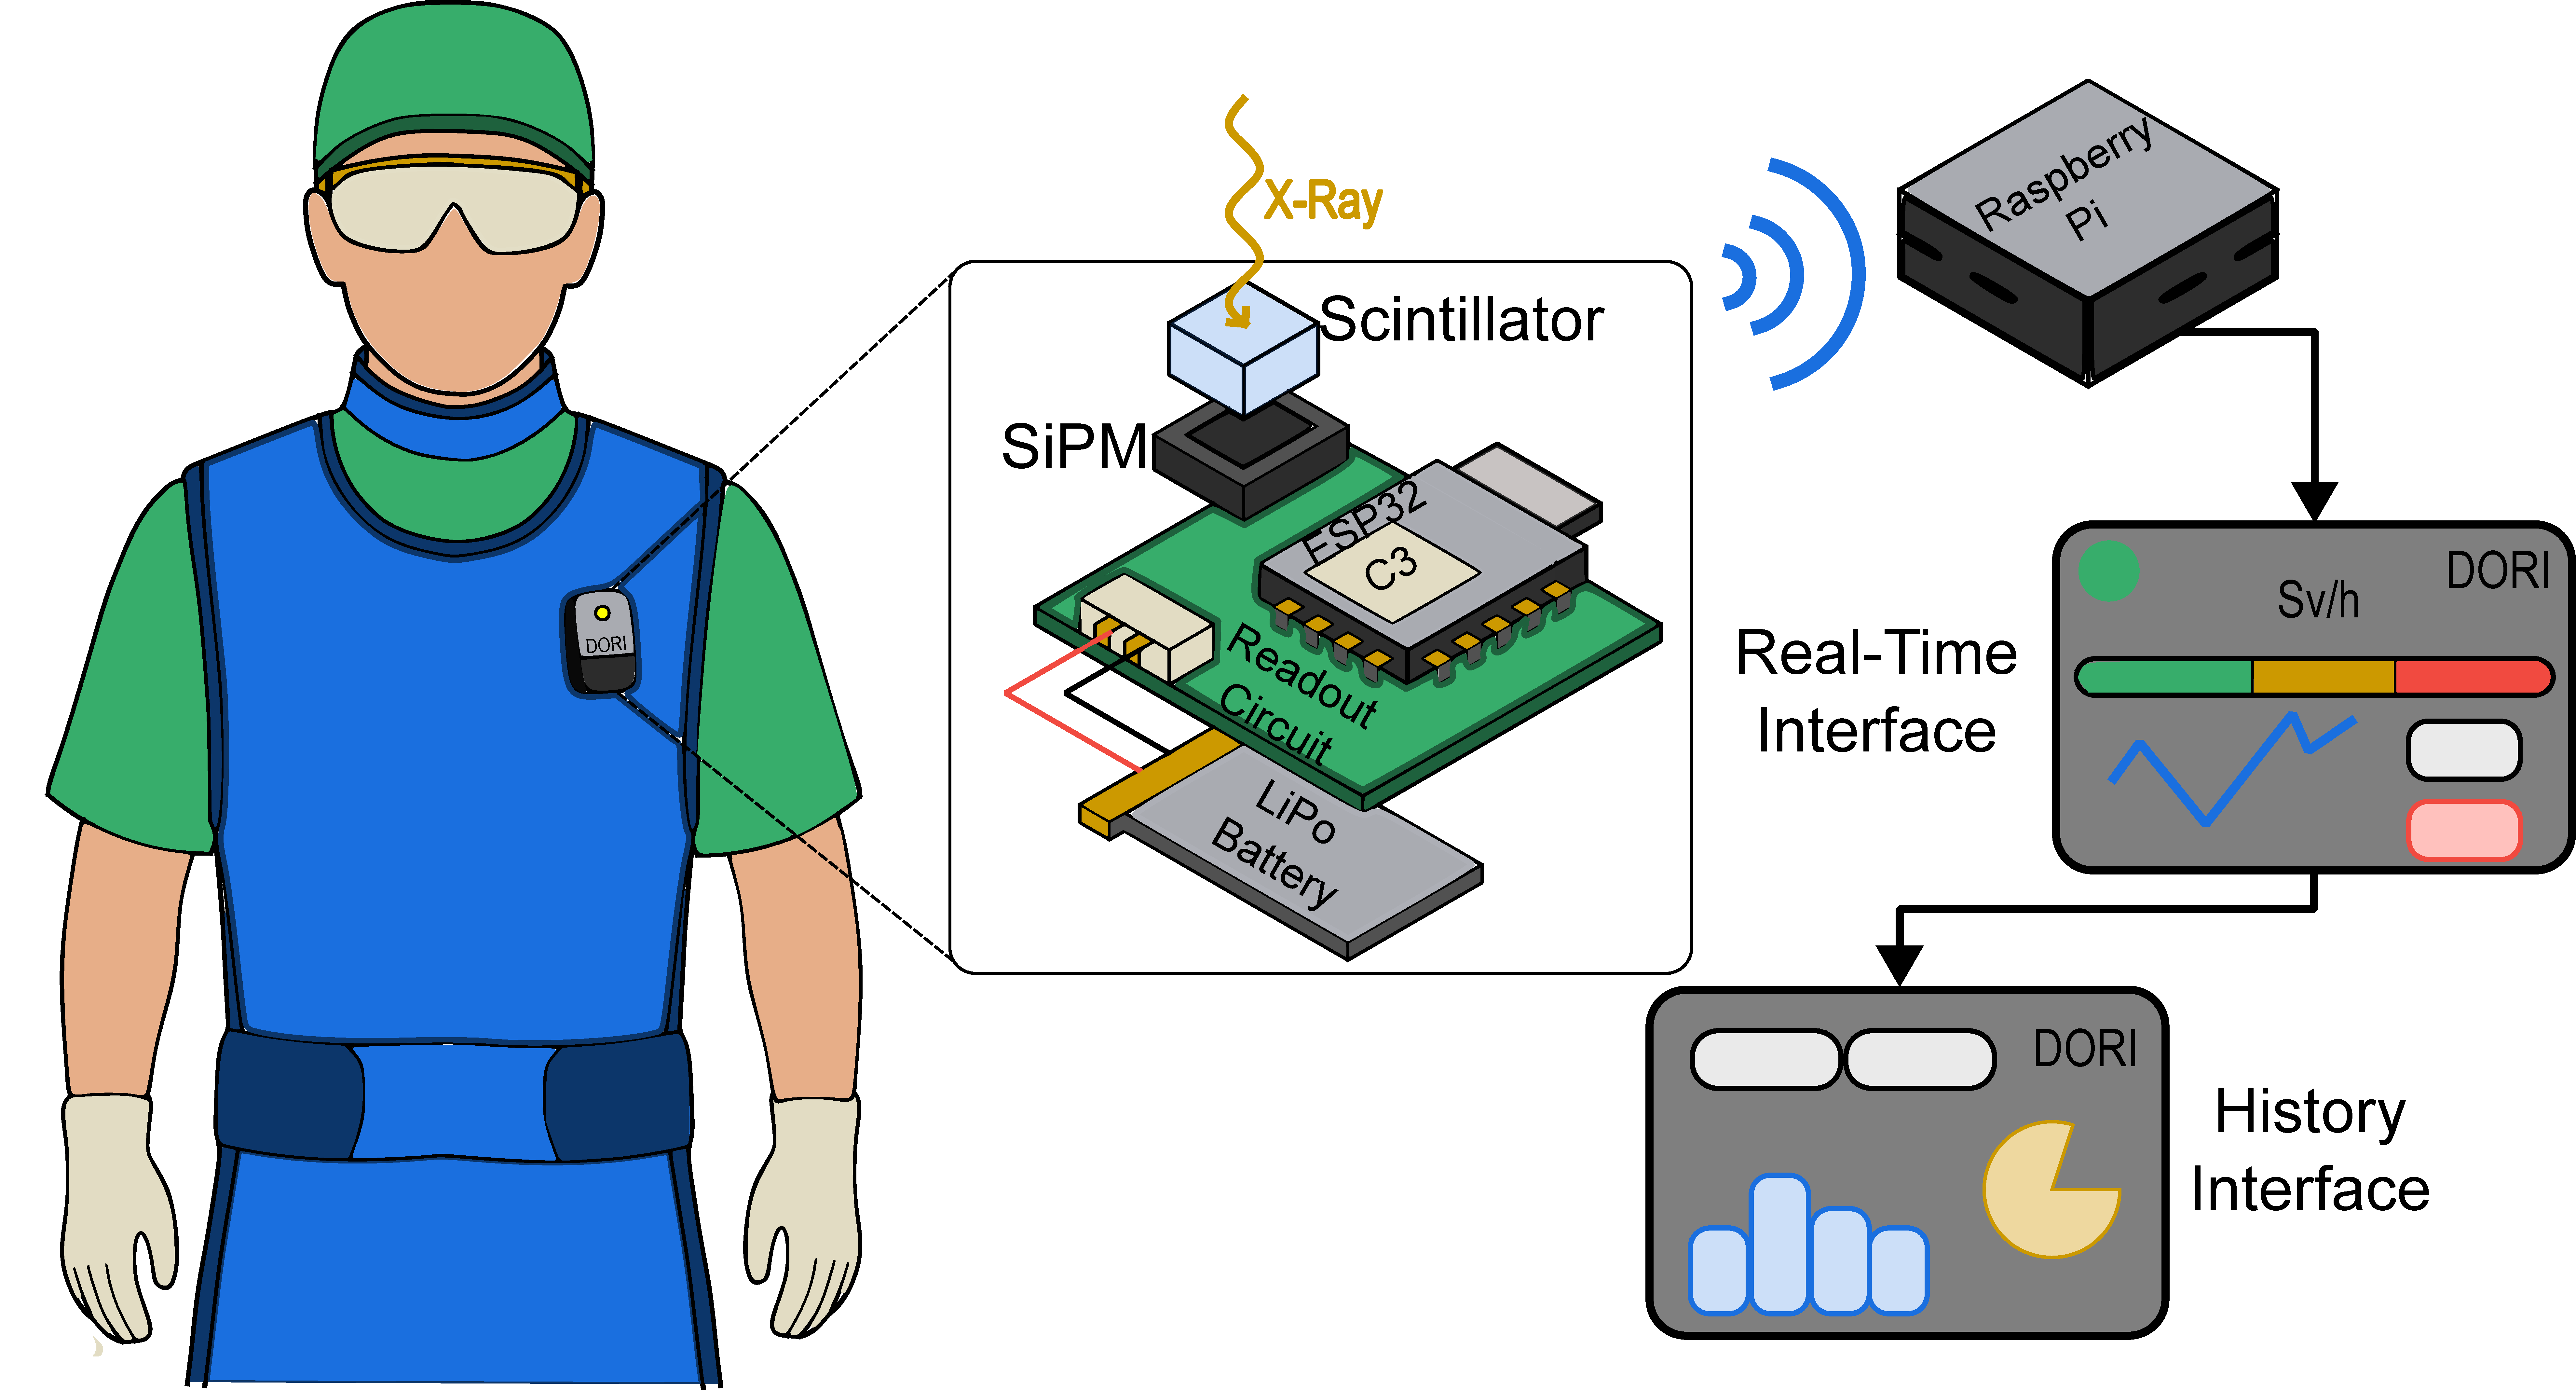
\includegraphics{images/DORI.pdf}}
  \end{center}
  \smallcap{The wearable unit (exploded view) is worn over the protective apron and comprises the scintillator, photodetector, readout circuit, MCU and LiPo battery. Data are sent to a Raspberry Pi, which displays the real-time and history interfaces.}
\end{frame}

% ---- fig:bias ----------------------------------------------------------
\begin{frame}
  \frametitle{SiPM Bias Supply}
  \begin{center}
    \adjustbox{max width=0.7\textwidth,max height=0.68\textheight}{\tikzset{every picture/.style={line width=0.75pt}} %set default line width to 0.75pt        

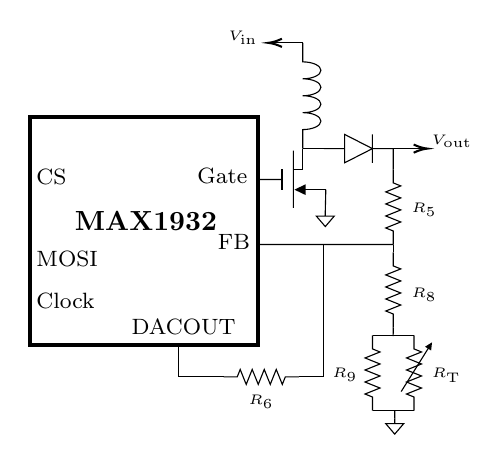
\begin{tikzpicture}[x=0.75pt,y=0.75pt,yscale=-1,xscale=1]
%uncomment if require: \path (0,300); %set diagram left start at 0, and has height of 300

%Shape: Square [id:dp45442051822513774] 
\draw  [line width=1.5]  (218.47,64.6) -- (328.47,64.6) -- (328.47,174.6) -- (218.47,174.6) -- cycle ;
%Shape: Inductor (Air Core) [id:dp8320962493713222] 
\draw   (350,29.04) -- (350,38.21) .. controls (354.83,38.21) and (358.75,40.04) .. (358.75,42.29) .. controls (358.75,44.54) and (354.83,46.37) .. (350,46.37) .. controls (354.83,46.37) and (358.75,48.19) .. (358.75,50.44) .. controls (358.75,52.69) and (354.83,54.52) .. (350,54.52) .. controls (354.83,54.52) and (358.75,56.35) .. (358.75,58.6) .. controls (358.75,60.85) and (354.83,62.67) .. (350,62.67) .. controls (354.83,62.67) and (358.75,64.5) .. (358.75,66.75) .. controls (358.75,69) and (354.83,70.83) .. (350,70.83) -- (350,80) ;
%Shape: Diode [id:dp522086168972487] 
\draw   (370.19,73.17) -- (383.57,80) -- (370.19,86.83) -- (370.19,73.17) -- cycle (360.16,80) -- (370.19,80) (383.57,73.17) -- (383.57,86.83) (383.57,80) -- (393.6,80) ;
%Shape: Resistor [id:dp8144600229276032] 
\draw   (393.61,90) -- (393.61,96.52) -- (397.22,97.97) -- (390,100.86) -- (397.22,103.76) -- (390,106.66) -- (397.22,109.55) -- (390,112.45) -- (397.22,115.35) -- (390,118.24) -- (393.61,119.69) -- (393.61,126.21) ;
%Straight Lines [id:da29049231672487486] 
\draw    (340,90) -- (340,100) ;
%Straight Lines [id:da4316288408593886] 
\draw    (361.11,99.78) -- (348.99,99.78) ;
\draw [shift={(345.99,99.78)}, rotate = 360] [fill={rgb, 255:red, 0; green, 0; blue, 0 }  ][line width=0.08]  [draw opacity=0] (5.36,-2.57) -- (0,0) -- (5.36,2.57) -- cycle    ;
%Straight Lines [id:da6953106373785519] 
\draw    (361.11,99.78) -- (360.86,110) ;
%Shape: Ground [id:dp011205472514209114] 
\draw   (356.54,112.52) -- (360.86,117.56) -- (365.17,112.52) -- (356.54,112.52) -- cycle (360.86,110) -- (360.86,112.52) ;
%Straight Lines [id:da5829290803316644] 
\draw    (350,80) -- (360.16,80) ;
%Straight Lines [id:da05768888846435982] 
\draw    (345.48,80.94) -- (345.5,108.61) ;
%Straight Lines [id:da31478243553340524] 
\draw    (350,80) -- (350,90) ;
%Straight Lines [id:da2330593515607322] 
\draw    (350,90) -- (345.79,90) ;
%Straight Lines [id:da3584287863409543] 
\draw    (328.59,94.89) -- (340.16,94.88) ;
%Shape: Resistor [id:dp4537216327878536] 
\draw   (393.61,130) -- (393.61,136.52) -- (397.22,137.97) -- (390,140.86) -- (397.22,143.76) -- (390,146.66) -- (397.22,149.55) -- (390,152.45) -- (397.22,155.35) -- (390,158.24) -- (393.61,159.69) -- (393.61,166.21) ;
%Shape: Resistor [id:dp44213159457902096] 
\draw   (383.61,170) -- (383.61,176.52) -- (387.22,177.97) -- (380,180.86) -- (387.22,183.76) -- (380,186.66) -- (387.22,189.55) -- (380,192.45) -- (387.22,195.35) -- (380,198.24) -- (383.61,199.69) -- (383.61,206.21) ;
%Shape: Resistor [id:dp5279058570816227] 
\draw   (403.61,170) -- (403.61,176.52) -- (407.22,177.97) -- (400,180.86) -- (407.22,183.76) -- (400,186.66) -- (407.22,189.55) -- (400,192.45) -- (407.22,195.35) -- (400,198.24) -- (403.61,199.69) -- (403.61,206.21) ;
%Shape: Ground [id:dp21864911769776485] 
\draw   (390,212.52) -- (394.31,217.56) -- (398.63,212.52) -- (390,212.52) -- cycle (394.31,210) -- (394.31,212.52) ;
%Shape: Resistor [id:dp5330487161197813] 
\draw   (311.9,190) -- (318.41,190) -- (319.86,186.39) -- (322.76,193.61) -- (325.65,186.39) -- (328.55,193.61) -- (331.45,186.39) -- (334.35,193.61) -- (337.24,186.39) -- (340.14,193.61) -- (341.59,190) -- (348.1,190) ;
%Straight Lines [id:da903277102568916] 
\draw    (397.43,197.05) -- (410.69,175.88) ;
\draw [shift={(412.29,173.33)}, rotate = 122.07] [fill={rgb, 255:red, 0; green, 0; blue, 0 }  ][line width=0.08]  [draw opacity=0] (3.57,-1.72) -- (0,0) -- (3.57,1.72) -- cycle    ;
%Straight Lines [id:da6627028399578476] 
\draw    (393.61,126.21) -- (393.61,130) ;
%Straight Lines [id:da19956176075595244] 
\draw    (383.61,170) -- (403.61,170) ;
%Straight Lines [id:da9867546245054489] 
\draw    (393.61,166.21) -- (393.56,170.39) ;
%Straight Lines [id:da699703638594996] 
\draw    (383.61,206.21) -- (403.61,206.21) ;
%Straight Lines [id:da6230017749012404] 
\draw    (394.3,206.05) -- (394.31,210) ;
%Straight Lines [id:da5942027422502576] 
\draw    (393.61,90) -- (393.6,80) ;
%Straight Lines [id:da7853613457386626] 
\draw    (393.61,126.21) -- (328.37,126.2) ;
%Straight Lines [id:da6727874772719629] 
\draw    (290,174.57) -- (290,190) ;
%Straight Lines [id:da9301720203284228] 
\draw    (311.9,190) -- (290,190) ;
%Straight Lines [id:da23173374113205025] 
\draw    (360,126.43) -- (360,190) ;
%Straight Lines [id:da39088728409946005] 
\draw    (348.1,190) -- (360,190) ;
%Straight Lines [id:da34090922258728096] 
\draw    (350,29.04) -- (335.39,29.04) ;
\draw [shift={(333.39,29.04)}, rotate = 360] [color={rgb, 255:red, 0; green, 0; blue, 0 }  ][line width=0.75]    (6.56,-1.97) .. controls (4.17,-0.84) and (1.99,-0.18) .. (0,0) .. controls (1.99,0.18) and (4.17,0.84) .. (6.56,1.97)   ;
%Straight Lines [id:da06307080945568311] 
\draw    (390,80) -- (408,80) ;
\draw [shift={(410,80)}, rotate = 180] [color={rgb, 255:red, 0; green, 0; blue, 0 }  ][line width=0.75]    (6.56,-1.97) .. controls (4.17,-0.84) and (1.99,-0.18) .. (0,0) .. controls (1.99,0.18) and (4.17,0.84) .. (6.56,1.97)   ;

% Text Node
\draw (298,88.22) node [anchor=north west][inner sep=0.75pt]  [font=\small] [align=left] {{\footnotesize Gate}};
% Text Node
\draw (307.9,120.17) node [anchor=north west][inner sep=0.75pt]  [font=\small] [align=left] {{\footnotesize FB}};
% Text Node
\draw (266.24,160.79) node [anchor=north west][inner sep=0.75pt]  [font=\small] [align=left] {{\footnotesize DACOUT}};
% Text Node
\draw (220.44,88.89) node [anchor=north west][inner sep=0.75pt]  [font=\small] [align=left] {{\footnotesize CS}};
% Text Node
\draw (220.44,128.33) node [anchor=north west][inner sep=0.75pt]  [font=\small] [align=left] {{\footnotesize MOSI}};
% Text Node
\draw (220.44,148.56) node [anchor=north west][inner sep=0.75pt]  [font=\small] [align=left] {{\footnotesize Clock}};
% Text Node
\draw (239,109) node [anchor=north west][inner sep=0.75pt]   [align=left] {\textbf{MAX1932}};
% Text Node
\draw (313,22) node [anchor=north west][inner sep=0.75pt]  [font=\tiny] [align=left] {$V_{\text{in}}$};
% Text Node
\draw (411,72) node [anchor=north west][inner sep=0.75pt]  [font=\tiny] [align=left] {$V_{\text{out}}$};
% Text Node
\draw (401.22,105.01) node [anchor=north west][inner sep=0.75pt]  [font=\tiny] [align=left] {$R_5$};
% Text Node
\draw (401.22,145.9) node [anchor=north west][inner sep=0.75pt]  [font=\tiny] [align=left] {$R_8$};
% Text Node
\draw (411,184.49) node [anchor=north west][inner sep=0.75pt]  [font=\tiny] [align=left] {$R_{\text{T}}$};
% Text Node
\draw (363,184.49) node [anchor=north west][inner sep=0.75pt]  [font=\tiny] [align=left] {$R_9$};
% Text Node
\draw (322.67,197.6) node [anchor=north west][inner sep=0.75pt]  [font=\tiny] [align=left] {$R_6$};

\end{tikzpicture}}
  \end{center}
  \smallcap{MAX1932 feedback network with the NTC thermistor $R_T$ for temperature compensation of the SiPM bias. Pin labels on the left correspond to SPI connections.}
\end{frame}

% ---- fig:architecture ---------------------------------------------------
\begin{frame}
  \frametitle{Architecture of the DORI System}
  \begin{center}
    \adjustbox{max width=0.96\textwidth,max height=0.72\textheight}{

\tikzset{every picture/.style={line width=0.75pt}} %set default line width to 0.75pt        

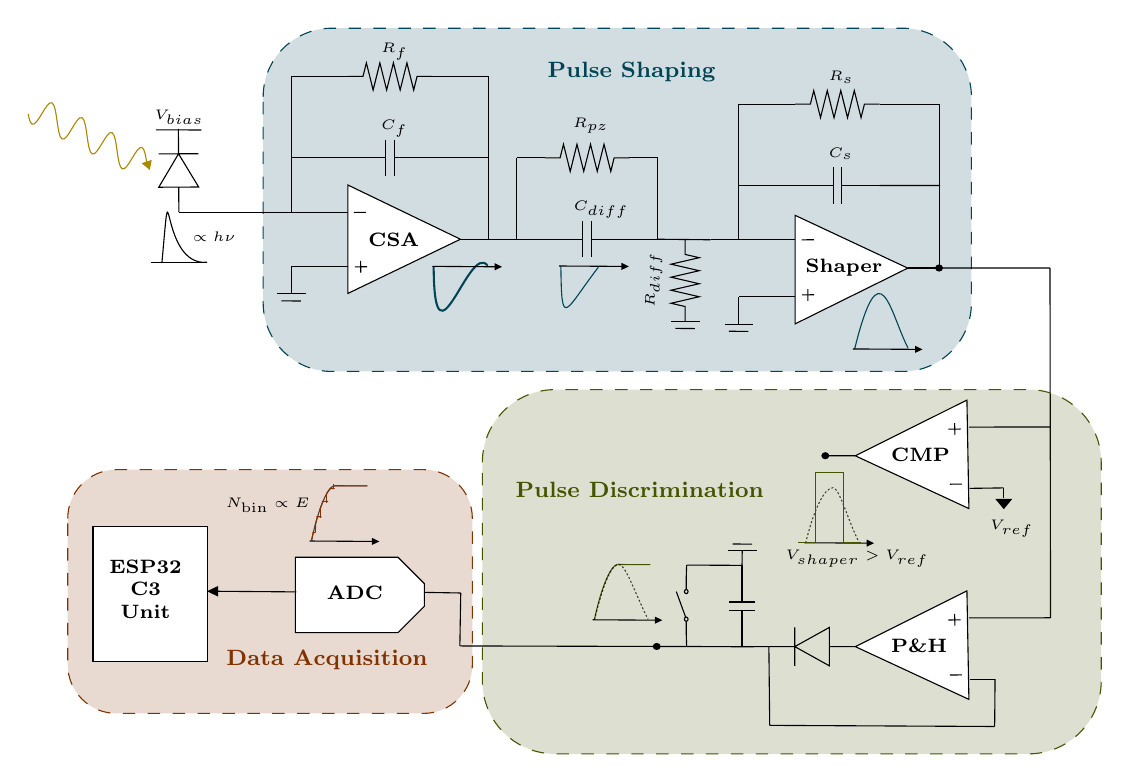
\begin{tikzpicture}[x=0.75pt,y=0.75pt,yscale=-1,xscale=1]
%uncomment if require: \path (0,390); %set diagram left start at 0, and has height of 390

%Rounded Rect [id:dp46800229916678826] 
\draw  [color={rgb, 255:red, 128; green, 51; blue, 0 }  ,draw opacity=1 ][fill={rgb, 255:red, 128; green, 51; blue, 0 }  ,fill opacity=0.18 ][dash pattern={on 4.5pt off 4.5pt}] (75.7,255.44) .. controls (75.7,242.46) and (86.22,231.95) .. (99.19,231.95) -- (247.14,231.95) .. controls (260.12,231.95) and (270.63,242.46) .. (270.63,255.44) -- (270.63,325.9) .. controls (270.63,338.88) and (260.12,349.39) .. (247.14,349.39) -- (99.19,349.39) .. controls (86.22,349.39) and (75.7,338.88) .. (75.7,325.9) -- cycle ;
%Rounded Rect [id:dp6060718292152891] 
\draw  [color={rgb, 255:red, 0; green, 68; blue, 85 }  ,draw opacity=1 ][fill={rgb, 255:red, 0; green, 68; blue, 85 }  ,fill opacity=0.18 ][dash pattern={on 4.5pt off 4.5pt}] (169.85,52.35) .. controls (169.85,34.09) and (184.66,19.28) .. (202.92,19.28) -- (478.01,19.28) .. controls (496.28,19.28) and (511.09,34.09) .. (511.09,52.35) -- (511.09,151.57) .. controls (511.09,169.84) and (496.28,184.64) .. (478.01,184.64) -- (202.92,184.64) .. controls (184.66,184.64) and (169.85,169.84) .. (169.85,151.57) -- cycle ;
%Straight Lines [id:da20418652663852965] 
\draw    (118.17,68.23) -- (140.04,68.31) ;
%Shape: Diode [id:dp9073484797643522] 
\draw   (119.56,95.88) -- (129.08,79.78) -- (138.77,95.78) -- (119.56,95.88) -- cycle (129.23,107.87) -- (129.17,95.83) (119.47,79.83) -- (138.68,79.73) (129.08,79.78) -- (129.01,67.74) ;
%Straight Lines [id:da29328469712985317] 
\draw    (129.23,107.87) -- (210.63,107.87) ;
%Shape: Triangle [id:dp7568885508488827] 
\draw  [fill={rgb, 255:red, 255; green, 255; blue, 255 }  ,fill opacity=1 ] (264.89,120.94) -- (210.63,147.08) -- (210.63,94.8) -- cycle ;
%Straight Lines [id:da4819348879555857] 
\draw    (210.63,134.01) -- (183.5,134.01) ;
%Straight Lines [id:da645749601403131] 
\draw    (183.5,147.08) -- (183.5,134.01) ;
%Straight Lines [id:da6803870332982462] 
\draw    (176.71,147.27) -- (190.28,147.27) ;
%Straight Lines [id:da005605298303441364] 
\draw    (178.65,150.63) -- (188.04,150.71) ;
%Straight Lines [id:da05308331089564988] 
\draw    (183.5,107.87) -- (183.5,81.73) ;
%Straight Lines [id:da020906030143946763] 
\draw    (183.5,42.51) -- (183.5,94.8) ;
%Shape: Resistor [id:dp7434947714198523] 
\draw   (210.63,42.51) -- (217.95,42.51) -- (219.58,35.98) -- (222.83,49.05) -- (226.09,35.98) -- (229.35,49.05) -- (232.6,35.98) -- (235.86,49.05) -- (239.11,35.98) -- (242.37,49.05) -- (244,42.51) -- (251.32,42.51) ;
%Shape: Capacitor [id:dp42145798620234975] 
\draw   (210.63,81.73) -- (228.94,81.73) (233.01,72.99) -- (233.01,90.46) (228.94,72.99) -- (228.94,90.46) (233.01,81.73) -- (251.32,81.73) ;
%Straight Lines [id:da34880193469214116] 
\draw    (210.63,42.51) -- (183.5,42.51) ;
%Straight Lines [id:da026503265572629386] 
\draw    (264.89,120.94) -- (292.02,120.94) ;
%Straight Lines [id:da9274117024294998] 
\draw    (278.45,42.51) -- (278.45,120.94) ;
%Straight Lines [id:da7747280381922488] 
\draw    (251.32,42.51) -- (278.45,42.51) ;
%Straight Lines [id:da1032408852686264] 
\draw    (183.5,81.73) -- (210.63,81.73) ;
%Straight Lines [id:da1423279487465121] 
\draw    (251.32,81.73) -- (278.45,81.73) ;
%Curve Lines [id:da7997259707368105] 
\draw [color={rgb, 255:red, 0; green, 0; blue, 0 }  ,draw opacity=1 ][fill={rgb, 255:red, 255; green, 255; blue, 255 }  ,fill opacity=1 ]   (121.09,132.03) .. controls (126.11,76.56) and (119.49,134.29) .. (142.8,132.03) ;
%Straight Lines [id:da9485003249156622] 
\draw    (115.67,132.03) -- (142.8,132.03) ;
%Curve Lines [id:da49583939836969093] 
\draw [color={rgb, 255:red, 0; green, 68; blue, 85 }  ,draw opacity=1 ]   (313.29,133.84) .. controls (313.63,164.72) and (314.85,155.96) .. (331.36,134.4) ;
%Shape: Resistor [id:dp18008683636522793] 
\draw   (305.58,81.73) -- (312.91,81.73) -- (314.54,75.19) -- (317.79,88.26) -- (321.05,75.19) -- (324.3,88.26) -- (327.56,75.19) -- (330.81,88.26) -- (334.07,75.19) -- (337.33,88.26) -- (338.95,81.73) -- (346.28,81.73) ;
%Straight Lines [id:da6245327821504196] 
\draw    (292.02,120.94) -- (292.02,81.73) ;
%Straight Lines [id:da9330542602485921] 
\draw    (292.02,81.73) -- (305.58,81.73) ;
%Straight Lines [id:da7057152830278173] 
\draw    (292.02,120.94) -- (305.58,120.94) ;
%Shape: Capacitor [id:dp8095550086511366] 
\draw   (305.58,120.94) -- (323.9,120.94) (327.97,112.21) -- (327.97,129.67) (323.9,112.21) -- (323.9,129.67) (327.97,120.94) -- (346.28,120.94) ;
%Straight Lines [id:da5386226934871385] 
\draw    (346.28,81.73) -- (359.84,81.73) ;
%Straight Lines [id:da7313083657794016] 
\draw    (346.28,120.94) -- (359.84,120.94) ;
%Straight Lines [id:da03131911441569635] 
\draw    (359.84,81.73) -- (359.84,120.94) ;
%Curve Lines [id:da7413273067238557] 
\draw [color={rgb, 255:red, 0; green, 68; blue, 85 }  ,draw opacity=1 ][line width=0.75]    (252,134.01) .. controls (252.17,187.85) and (269.17,121.74) .. (278,133.68) ;
%Shape: Triangle [id:dp6184826935280519] 
\draw  [fill={rgb, 255:red, 255; green, 255; blue, 255 }  ,fill opacity=1 ] (480.43,134.86) -- (426.17,161.72) -- (426.17,109.44) -- cycle ;
%Straight Lines [id:da31773246729249327] 
\draw    (426.17,148.65) -- (399.03,148.65) ;
%Straight Lines [id:da3550332613541024] 
\draw    (399.03,161.72) -- (399.03,148.65) ;
%Straight Lines [id:da8025351063037379] 
\draw    (392.25,161.91) -- (405.82,161.91) ;
%Straight Lines [id:da02403217066549712] 
\draw    (394.19,165.27) -- (403.58,165.35) ;
%Straight Lines [id:da16841076045424963] 
\draw    (385.47,121.2) -- (426.17,121.2) ;
%Straight Lines [id:da5746709989474186] 
\draw    (399.03,121.2) -- (399.03,95.06) ;
%Straight Lines [id:da2718623980119098] 
\draw    (399.03,55.84) -- (399.03,108.13) ;
%Shape: Resistor [id:dp29501269522921625] 
\draw   (426.17,55.84) -- (433.49,55.84) -- (435.12,49.31) -- (438.37,62.38) -- (441.63,49.31) -- (444.89,62.38) -- (448.14,49.31) -- (451.4,62.38) -- (454.65,49.31) -- (457.91,62.38) -- (459.54,55.84) -- (466.86,55.84) ;
%Shape: Capacitor [id:dp6295648569904636] 
\draw   (426.17,95.06) -- (444.48,95.06) (448.55,86.32) -- (448.55,103.79) (444.48,86.32) -- (444.48,103.79) (448.55,95.06) -- (466.86,95.06) ;
%Straight Lines [id:da39447831240426734] 
\draw    (426.17,55.84) -- (399.03,55.84) ;
%Straight Lines [id:da7401181488947025] 
\draw    (548.94,134.81) -- (549.21,303.33) ;
%Straight Lines [id:da3780881206944031] 
\draw    (466.86,55.84) -- (495.5,55.84) ;
%Straight Lines [id:da4232645895231355] 
\draw    (399.03,95.06) -- (426.17,95.06) ;
%Straight Lines [id:da4266027647624573] 
\draw    (466.86,95.06) -- (495.95,95.05) ;
%Straight Lines [id:da5672944700293289] 
\draw    (480.43,134.8) -- (495.5,134.8) ;
%Straight Lines [id:da469893720694727] 
\draw    (213.52,108.04) -- (219.36,107.98) ;
%Straight Lines [id:da9392787125105846] 
\draw    (251.32,134.01) -- (281.93,134.21) ;
\draw [shift={(284.93,134.23)}, rotate = 180.37] [fill={rgb, 255:red, 0; green, 0; blue, 0 }  ][line width=0.08]  [draw opacity=0] (3.57,-1.72) -- (0,0) -- (3.57,1.72) -- cycle    ;
%Straight Lines [id:da6932257001220354] 
\draw    (312.44,133.84) -- (343.05,134.03) ;
\draw [shift={(346.05,134.05)}, rotate = 180.37] [fill={rgb, 255:red, 0; green, 0; blue, 0 }  ][line width=0.08]  [draw opacity=0] (3.57,-1.72) -- (0,0) -- (3.57,1.72) -- cycle    ;
%Straight Lines [id:da6166140138845793] 
\draw    (214.06,134.25) -- (219.9,134.19) ;
%Shape: Boxed Line [id:dp7328235768970041] 
\draw    (216.82,131.4) -- (216.87,137.02) ;
%Straight Lines [id:da9592107478171705] 
\draw    (429.33,121.24) -- (435.17,121.18) ;
%Shape: Boxed Line [id:dp06578186279615383] 
\draw    (432.26,145) -- (432.31,150.63) ;
%Straight Lines [id:da21273186496269592] 
\draw    (429.48,147.76) -- (435.31,147.69) ;
%Shape: Resistor [id:dp07090411488435666] 
\draw   (373.14,121.2) -- (373.14,128.26) -- (379.92,129.83) -- (366.35,132.97) -- (379.92,136.1) -- (366.35,139.24) -- (379.92,142.38) -- (366.35,145.51) -- (379.92,148.65) -- (366.35,151.79) -- (373.14,153.36) -- (373.14,160.42) ;
%Straight Lines [id:da5181129573733605] 
\draw    (366.56,160.54) -- (380.13,160.54) ;
%Straight Lines [id:da36868876671547046] 
\draw    (368.5,163.9) -- (377.89,163.98) ;
%Straight Lines [id:da4086711222947753] 
\draw    (359.84,120.94) -- (385.47,121.2) ;
%Rounded Rect [id:dp3460824200505386] 
\draw  [color={rgb, 255:red, 68; green, 85; blue, 0 }  ,draw opacity=1 ][fill={rgb, 255:red, 68; green, 85; blue, 0 }  ,fill opacity=0.18 ][dash pattern={on 4.5pt off 4.5pt}] (275.46,228.49) .. controls (275.46,209.1) and (291.18,193.39) .. (310.56,193.39) -- (538.52,193.39) .. controls (557.91,193.39) and (573.62,209.1) .. (573.62,228.49) -- (573.62,333.79) .. controls (573.62,353.18) and (557.91,368.89) .. (538.52,368.89) -- (310.56,368.89) .. controls (291.18,368.89) and (275.46,353.18) .. (275.46,333.79) -- cycle ;
%Shape: Triangle [id:dp21057859356469377] 
\draw  [fill={rgb, 255:red, 255; green, 255; blue, 255 }  ,fill opacity=1 ] (455.14,225.28) -- (508.92,198.42) -- (509.87,250.71) -- cycle ;
%Straight Lines [id:da7294664906139928] 
\draw    (506.48,238.91) -- (500.65,238.97) ;
%Shape: Boxed Line [id:dp3537895946781868] 
\draw    (503.13,215.14) -- (502.98,209.52) ;
%Straight Lines [id:da9669577971099538] 
\draw    (505.86,212.39) -- (500.02,212.45) ;
%Straight Lines [id:da8006808934622864] 
\draw    (510.26,240.97) -- (526.57,240.75) ;
%Shape: Triangle [id:dp4851626389643716] 
\draw  [fill={rgb, 255:red, 0; green, 0; blue, 0 }  ,fill opacity=1 ] (526.69,250.57) -- (523.14,246.29) -- (530.24,246.29) -- cycle ;
%Straight Lines [id:da7399314250868523] 
\draw    (455.14,225.28) -- (440.69,225.25) ;
%Flowchart: Connector [id:dp3531466314065995] 
\draw  [fill={rgb, 255:red, 0; green, 0; blue, 0 }  ,fill opacity=1 ] (493.88,134.8) .. controls (493.88,134) and (494.61,133.35) .. (495.5,133.35) .. controls (496.39,133.35) and (497.11,134) .. (497.11,134.8) .. controls (497.11,135.59) and (496.39,136.24) .. (495.5,136.24) .. controls (494.61,136.24) and (493.88,135.59) .. (493.88,134.8) -- cycle ;
%Straight Lines [id:da9446115204522941] 
\draw    (509.88,211.45) -- (549.21,211.39) ;
%Curve Lines [id:da31175352604231354] 
\draw [color={rgb, 255:red, 0; green, 68; blue, 85 }  ,draw opacity=1 ]   (454.82,173.8) .. controls (467.17,123.88) and (471.61,155.96) .. (480.63,173.55) ;
%Straight Lines [id:da8734375505712497] 
\draw    (453.91,173.8) -- (484.52,174) ;
\draw [shift={(487.51,174.02)}, rotate = 180.37] [fill={rgb, 255:red, 0; green, 0; blue, 0 }  ][line width=0.08]  [draw opacity=0] (3.57,-1.72) -- (0,0) -- (3.57,1.72) -- cycle    ;
%Straight Lines [id:da6007611642847911] 
\draw    (430.57,267.17) -- (461.17,267.37) ;
\draw [shift={(464.17,267.38)}, rotate = 180.37] [fill={rgb, 255:red, 0; green, 0; blue, 0 }  ][line width=0.08]  [draw opacity=0] (3.57,-1.72) -- (0,0) -- (3.57,1.72) -- cycle    ;
%Curve Lines [id:da5409343504904985] 
\draw [color={rgb, 255:red, 0; green, 0; blue, 0 }  ,draw opacity=0.7 ] [dash pattern={on 0.75pt off 0.75pt on 0.75pt off 0.75pt}]  (431.19,267.37) .. controls (436.14,247.38) and (441.17,240.57) .. (444.39,240.68) .. controls (447.6,240.8) and (451.6,256.57) .. (457.01,267.12) ;
%Shape: Pulse Wave Form [id:dp37814170861699237] 
\draw  [color={rgb, 255:red, 68; green, 85; blue, 0 }  ,draw opacity=1 ] (427.44,267.23) -- (435.91,267.23) -- (435.91,233.36) -- (449.48,233.36) -- (449.48,267.23) -- (457.96,267.23) ;

%Straight Lines [id:da8033158731026477] 
\draw    (328.55,304.29) -- (359.16,304.48) ;
\draw [shift={(362.16,304.5)}, rotate = 180.37] [fill={rgb, 255:red, 0; green, 0; blue, 0 }  ][line width=0.08]  [draw opacity=0] (3.57,-1.72) -- (0,0) -- (3.57,1.72) -- cycle    ;
%Curve Lines [id:da8165839321439692] 
\draw [color={rgb, 255:red, 68; green, 85; blue, 0 }  ,draw opacity=1 ]   (329.46,304.29) .. controls (330.89,296.83) and (335.71,278.62) .. (340.54,277.66) ;
%Straight Lines [id:da9249993527350234] 
\draw [color={rgb, 255:red, 68; green, 85; blue, 0 }  ,draw opacity=1 ]   (340.54,277.66) -- (356.36,277.74) ;
%Curve Lines [id:da01278581006202073] 
\draw [color={rgb, 255:red, 0; green, 0; blue, 0 }  ,draw opacity=0.7 ] [dash pattern={on 0.75pt off 0.75pt on 0.75pt off 0.75pt}]  (329.46,304.29) .. controls (334.41,284.3) and (338.09,277.46) .. (341.3,277.57) .. controls (344.51,277.68) and (349.87,293.49) .. (355.27,304.04) ;
%Straight Lines [id:da36645697031500035] 
\draw    (526.57,245.78) -- (526.57,240.75) ;
%Shape: Triangle [id:dp48501946316287736] 
\draw  [fill={rgb, 255:red, 255; green, 255; blue, 255 }  ,fill opacity=1 ] (455.14,317.22) -- (508.92,290.36) -- (509.87,342.64) -- cycle ;
%Straight Lines [id:da6036906170346914] 
\draw    (506.48,330.84) -- (500.65,330.91) ;
%Shape: Boxed Line [id:dp6726482576478763] 
\draw    (503.13,307.08) -- (502.98,301.45) ;
%Straight Lines [id:da037444841152633135] 
\draw    (505.86,304.32) -- (500.02,304.39) ;
%Straight Lines [id:da5709459533271122] 
\draw    (510.26,332.91) -- (522.47,332.91) ;
%Straight Lines [id:da19356976941121384] 
\draw    (509.88,303.38) -- (549.21,303.33) ;
%Shape: Diode [id:dp614316518769653] 
\draw   (442.65,326.48) -- (425.99,317.22) -- (442.65,307.96) -- (442.65,326.48) -- cycle (455.14,317.22) -- (442.65,317.22) (425.99,326.48) -- (425.99,307.96) (425.99,317.22) -- (413.5,317.22) ;
%Straight Lines [id:da09813703953082598] 
\draw    (413.5,317.22) -- (413.9,355.16) ;
%Straight Lines [id:da849214487415646] 
\draw    (413.9,355.16) -- (522.28,355.7) ;
%Straight Lines [id:da125511136072201] 
\draw    (522.47,332.91) -- (522.28,355.7) ;
%Shape: Capacitor [id:dp7142356900456059] 
\draw   (400.56,278.07) -- (400.56,295.71) (407,299.63) -- (394.12,299.63) (407,295.71) -- (394.12,295.71) (400.56,299.63) -- (400.56,317.28) ;
%Shape: Simple Switch [id:dp5297728261178234] 
\draw   (373.67,310.11) -- (373.67,305) (373.67,289.68) -- (373.67,284.57) (373.37,302.96) -- (368.9,290.7) (373.67,291.72) .. controls (373.18,291.72) and (372.78,291.26) .. (372.78,290.7) .. controls (372.78,290.14) and (373.18,289.68) .. (373.67,289.68) .. controls (374.17,289.68) and (374.57,290.14) .. (374.57,290.7) .. controls (374.57,291.26) and (374.17,291.72) .. (373.67,291.72) -- cycle (373.67,305) .. controls (373.18,305) and (372.78,304.54) .. (372.78,303.98) .. controls (372.78,303.42) and (373.18,302.96) .. (373.67,302.96) .. controls (374.17,302.96) and (374.57,303.42) .. (374.57,303.98) .. controls (374.57,304.54) and (374.17,305) .. (373.67,305) -- cycle ;
%Straight Lines [id:da9962880185364887] 
\draw    (400.56,278.07) -- (373.87,277.93) ;
%Straight Lines [id:da4168400592441782] 
\draw    (400.56,317.28) -- (373.87,317.15) ;
%Straight Lines [id:da6629627230865746] 
\draw    (373.87,277.93) -- (373.67,284.57) ;
%Straight Lines [id:da6227335867281195] 
\draw    (373.67,310.11) -- (373.87,317.15) ;
%Straight Lines [id:da9440197749138511] 
\draw    (400.56,317.28) -- (413.5,317.22) ;
%Straight Lines [id:da5574398837436616] 
\draw    (373.87,317.15) -- (359.47,317.14) ;
%Flowchart: Connector [id:dp28586564232252365] 
\draw  [fill={rgb, 255:red, 0; green, 0; blue, 0 }  ,fill opacity=1 ] (439.08,225.25) .. controls (439.08,224.45) and (439.8,223.81) .. (440.69,223.81) .. controls (441.58,223.81) and (442.3,224.45) .. (442.3,225.25) .. controls (442.3,226.05) and (441.58,226.69) .. (440.69,226.69) .. controls (439.8,226.69) and (439.08,226.05) .. (439.08,225.25) -- cycle ;
%Flowchart: Connector [id:dp5135507227534388] 
\draw  [fill={rgb, 255:red, 0; green, 0; blue, 0 }  ,fill opacity=1 ] (357.86,317.14) .. controls (357.86,316.35) and (358.58,315.7) .. (359.47,315.7) .. controls (360.36,315.7) and (361.08,316.35) .. (361.08,317.14) .. controls (361.08,317.94) and (360.36,318.58) .. (359.47,318.58) .. controls (358.58,318.58) and (357.86,317.94) .. (357.86,317.14) -- cycle ;
%Shape: Wave [id:dp059927494842615836] 
\draw  [color={rgb, 255:red, 170; green, 136; blue, 0 }  ,draw opacity=1 ] (56.66,60.65) .. controls (57.1,63.11) and (57.63,65.03) .. (58.51,65.46) .. controls (59.82,66.11) and (61.52,63.3) .. (63.3,60.33) .. controls (65.08,57.37) and (66.78,54.56) .. (68.09,55.21) .. controls (69.4,55.86) and (69.96,59.8) .. (70.54,63.93) .. controls (71.12,68.06) and (71.67,72) .. (72.98,72.65) .. controls (74.29,73.3) and (75.99,70.48) .. (77.77,67.52) .. controls (79.55,64.56) and (81.25,61.75) .. (82.56,62.4) .. controls (83.87,63.05) and (84.43,66.98) .. (85,71.12) .. controls (85.58,75.25) and (86.14,79.19) .. (87.45,79.84) .. controls (88.76,80.49) and (90.46,77.67) .. (92.24,74.71) .. controls (94.02,71.75) and (95.72,68.94) .. (97.03,69.59) .. controls (98.34,70.24) and (98.89,74.17) .. (99.47,78.31) .. controls (100.05,82.44) and (100.61,86.38) .. (101.92,87.03) .. controls (103.23,87.68) and (104.93,84.86) .. (106.71,81.9) .. controls (108.49,78.94) and (110.19,76.12) .. (111.5,76.77) .. controls (112.71,77.37) and (113.27,80.78) .. (113.81,84.55) ;
%Shape: Triangle [id:dp3108622029974263] 
\draw  [color={rgb, 255:red, 170; green, 136; blue, 0 }  ,draw opacity=1 ][fill={rgb, 255:red, 170; green, 136; blue, 0 }  ,fill opacity=1 ] (115.05,87.07) -- (111.86,84.44) -- (115.81,83.09) -- cycle ;
%Straight Lines [id:da5842921754561695] 
\draw    (400.56,278.07) -- (400.66,271.23) ;
%Straight Lines [id:da97191101904161] 
\draw    (396,267.77) -- (400.92,267.81) -- (405.39,267.84) ;
%Straight Lines [id:da8202699426795026] 
\draw    (393.99,271.03) -- (395.72,271.03) -- (407.56,271.03) ;
%Snip Same Side Corner Rect [id:dp24267720786095204] 
\draw  [fill={rgb, 255:red, 255; green, 255; blue, 255 }  ,fill opacity=1 ] (234.8,274.15) -- (247.52,286.87) -- (247.52,297.77) -- (234.8,310.49) -- (185.39,310.49) -- (185.39,310.49) -- (185.39,274.15) -- (185.39,274.15) -- cycle ;
%Shape: Rectangle [id:dp4960716974860516] 
\draw  [fill={rgb, 255:red, 255; green, 255; blue, 255 }  ,fill opacity=1 ] (87.86,259.38) -- (142.94,259.38) -- (142.94,324.22) -- (87.86,324.22) -- cycle ;
%Straight Lines [id:da5259235282088736] 
\draw    (264.62,316.89) -- (359.47,317.14) ;
%Straight Lines [id:da04918323557857496] 
\draw    (247.85,291.09) -- (265.04,291.38) ;
%Straight Lines [id:da700345769463564] 
\draw    (265.04,291.38) -- (264.62,316.89) ;
%Straight Lines [id:da44513384727711636] 
\draw    (192.21,266.34) -- (222.82,266.54) ;
\draw [shift={(225.82,266.56)}, rotate = 180.37] [fill={rgb, 255:red, 0; green, 0; blue, 0 }  ][line width=0.08]  [draw opacity=0] (3.57,-1.72) -- (0,0) -- (3.57,1.72) -- cycle    ;
%Curve Lines [id:da06577028557977793] 
\draw [color={rgb, 255:red, 0; green, 0; blue, 0 }  ,draw opacity=0.7 ]   (193.12,266.34) .. controls (194.55,258.88) and (199.36,240.67) .. (204.19,239.71) ;
%Straight Lines [id:da0572237289311508] 
\draw [color={rgb, 255:red, 0; green, 0; blue, 0 }  ,draw opacity=0.7 ]   (204.19,239.71) -- (220.01,239.8) ;
%Curve Lines [id:da3804043288541633] 
\draw [color={rgb, 255:red, 128; green, 51; blue, 0 }  ,draw opacity=1 ] [dash pattern={on 3pt off 3pt on 3pt off 3pt}]  (193.12,266.34) .. controls (194.55,258.88) and (199.36,240.67) .. (204.19,239.71) ;
%Straight Lines [id:da5333998307295363] 
\draw [color={rgb, 255:red, 128; green, 51; blue, 0 }  ,draw opacity=1 ]   (193.63,262.21) -- (195,262.32) ;
%Straight Lines [id:da40393427405433224] 
\draw [color={rgb, 255:red, 128; green, 51; blue, 0 }  ,draw opacity=1 ]   (195,262.32) -- (195.08,258.23) ;
%Straight Lines [id:da3824884565346163] 
\draw [color={rgb, 255:red, 128; green, 51; blue, 0 }  ,draw opacity=1 ]   (202.04,241.08) -- (204.32,241.09) ;
%Straight Lines [id:da8760345808356574] 
\draw [color={rgb, 255:red, 128; green, 51; blue, 0 }  ,draw opacity=1 ]   (203.75,241.36) -- (203.75,239.04) ;

%Straight Lines [id:da012864593156911797] 
\draw [color={rgb, 255:red, 128; green, 51; blue, 0 }  ,draw opacity=1 ]   (195.47,254.61) -- (197.96,254.68) ;
%Straight Lines [id:da7563678124476333] 
\draw [color={rgb, 255:red, 128; green, 51; blue, 0 }  ,draw opacity=1 ]   (197.4,255.23) -- (197.4,250.54) ;
%Straight Lines [id:da5333243365793827] 
\draw [color={rgb, 255:red, 128; green, 51; blue, 0 }  ,draw opacity=1 ]   (198.85,247.27) -- (198.18,247.22) -- (201.13,247.28) ;
%Straight Lines [id:da6175946543817453] 
\draw [color={rgb, 255:red, 128; green, 51; blue, 0 }  ,draw opacity=1 ]   (200.56,247.82) -- (200.56,247.22) -- (200.56,243.14) ;
%Straight Lines [id:da3521344691026579] 
\draw [color={rgb, 255:red, 128; green, 51; blue, 0 }  ,draw opacity=1 ]   (204.19,239.71) -- (220.01,239.8) ;
%Straight Lines [id:da18368526561352316] 
\draw    (185.87,290.85) -- (145.8,290.54) ;
\draw [shift={(142.8,290.52)}, rotate = 0.43] [fill={rgb, 255:red, 0; green, 0; blue, 0 }  ][line width=0.08]  [draw opacity=0] (5.36,-2.57) -- (0,0) -- (5.36,2.57) -- cycle    ;
%Straight Lines [id:da56033182920969] 
\draw    (495.5,55.84) -- (495.5,133.35) ;
%Straight Lines [id:da784442544187718] 
\draw    (495.5,134.8) -- (548.94,134.81) ;

% Text Node
\draw (225.47,25.29) node [anchor=north west][inner sep=0.75pt]  [font=\tiny] [align=left] {$R_{f}$};
% Text Node
\draw (225.47,62.28) node [anchor=north west][inner sep=0.75pt]  [font=\tiny] [align=left] {$C_{f}$};
% Text Node
\draw (116.3,57.49) node [anchor=north west][inner sep=0.75pt]  [font=\tiny] [align=left] {$V_{bias}$};
% Text Node
\draw (134.54,116.18) node [anchor=north west][inner sep=0.75pt] [font=\tiny] {\(\propto h\nu\)};
% Text Node
\draw (317.75,61.5) node [anchor=north west][inner sep=0.75pt]  [font=\tiny] [align=left] {$R_{pz}$};
% Text Node
\draw (318.11,101.49) node [anchor=north west][inner sep=0.75pt]  [font=\tiny] [align=left] {$C_{diff}$};
% Text Node
\draw (441.01,38.62) node [anchor=north west][inner sep=0.75pt]  [font=\tiny] [align=left] {$R_{s}$};
% Text Node
\draw (441.01,75.61) node [anchor=north west][inner sep=0.75pt]  [font=\tiny] [align=left] {$C_{s}$};
% Text Node
\draw (219.33,116.63) node [anchor=north west][inner sep=0.75pt]  [font=\scriptsize] [align=left] {{\scriptsize \textbf{CSA}}};
% Text Node
\draw (430,129) node [anchor=north west][inner sep=0.75pt]  [font=\scriptsize] [align=left] {{\scriptsize \textbf{Shaper}}};
% Text Node
\draw (305.69,34.53) node [anchor=north west][inner sep=0.75pt]   [align=left] {\textbf{{\footnotesize \textcolor[rgb]{0,0.27,0.33}{Pulse Shaping}}}};
% Text Node
\draw (352.68,155.01) node [anchor=north west][inner sep=0.75pt]  [font=\tiny,rotate=-270] [align=left] {$R_{diff}$};
% Text Node
\draw (518.87,255.11) node [anchor=north west][inner sep=0.75pt]  [font=\tiny] [align=left] {$V_{ref}$};
% Text Node
\draw (471.18,220.38) node [anchor=north west][inner sep=0.75pt]  [font=\scriptsize] [align=left] {{\scriptsize \textbf{CMP}}};
% Text Node
\draw (420.26,269.33) node [anchor=north west][inner sep=0.75pt]   [align=left] {{\tiny $V_{shaper} > V_{ref}$}};
% Text Node
\draw (471.18,312.13) node [anchor=north west][inner sep=0.75pt]  [font=\scriptsize] [align=left] {{\scriptsize \textbf{P\&H}}};
% Text Node
\draw (290.23,236.5) node [anchor=north west][inner sep=0.75pt]   [align=left] {\textbf{{\footnotesize \textcolor[rgb]{0.27,0.33,0}{Pulse Discrimination}}}};
% Text Node
\draw (199.34,286.87) node [anchor=north west][inner sep=0.75pt]  [font=\scriptsize] [align=left] {{\scriptsize \textbf{ADC}}};
% Text Node
\draw (94.49,274.48) node [anchor=north west][inner sep=0.75pt] [font=\scriptsize] [align=center] {
\textbf{ESP32}\\
\textbf{C3}\\
\textbf{Unit}
};
% Text Node
\draw (150.9,317.64) node [anchor=north west][inner sep=0.75pt]   [align=left] {\textbf{{\footnotesize \textcolor[rgb]{0.5,0.2,0}{Data Acquisition}}}};
% Text Node
\draw (150.67,244.28) node [anchor=north west][inner sep=0.75pt]  [font=\tiny] [align=left] {$N_{\text{bin}} \propto E$};

\end{tikzpicture}


}
  \end{center}
\end{frame}

% ---- fig:pcb -------------------------------------------------------------
\begin{frame}
  \frametitle{DORI-Test Board}
  \begin{center}
    \begin{minipage}[c]{0.52\linewidth}
      \centering
      \adjustbox{max width=\linewidth,max height=0.55\textheight}{\begin{tikzpicture}[x=1pt,y=1pt,
    every node/.style={font=\footnotesize},
    ah/.style={draw opacity=0,line width=0.08,fill opacity=1},
    lbl/.style={fill=white,align=center,inner sep=2.5pt,line width=0.6pt},
    dim/.style={fill=white,align=center,inner sep=2pt,draw=none,font=\scriptsize},
    reg/.style={line width=1.2pt}]

% ---- Photograph -------------------------------------------------------
\node [anchor=south west,inner sep=0] at (0,0)
  {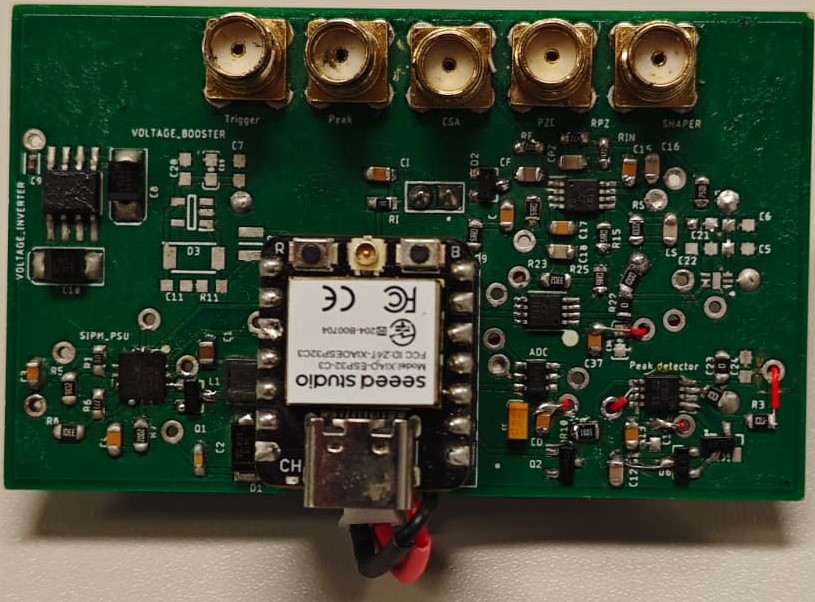
\includegraphics[width=186pt,height=127pt]{images/pcb_teste.jpg}};

% ---- Region outlines ---------------------------------------------------
\draw [reg,color={rgb, 255:red, 241; green, 74; blue, 64 }]
      (2.55,24.84) rectangle (52.93,59.98);                 % SiPM power supply
\draw [reg,color={rgb, 255:red, 26; green, 111; blue, 223 }]
      (116.09,72.67) rectangle (166.47,101.07);             % pulse shaping
\draw [reg,color={rgb, 255:red, 204; green, 153; blue, 0 }]
      (113.63,34.27) rectangle (129.67,53.47);              % ADC
\draw [reg,color={rgb, 255:red, 55; green, 173; blue, 107 }]
      (113.51,63.72) .. controls (118.22,73.60) and (139.09,68.88) .. (153.45,57.88)
   .. controls (167.81,46.87) and (177.68,49.12) .. (178.35,43.95)
   .. controls (179.03,38.79) and (182.39,38.56) .. (172.97,30.48)
   .. controls (163.55,22.40) and (163.98,22.18) .. (151.65,21.95)
   .. controls (139.33,21.72) and (126.97,19.26) .. (126.86,25.54)
   .. controls (126.74,31.83) and (140.14,43.95) .. (136.62,50.01)
   .. controls (133.10,56.08) and (108.80,53.84) .. (113.51,63.72) -- cycle ;

% ---- Labels over the board (no arrows) --------------------------------
\node [lbl,draw=none,font=\scriptsize,anchor=center] at (83.33,54.66) {MCU};
\node [lbl,draw={rgb, 255:red, 204; green, 153; blue, 0 },
       font=\scriptsize,anchor=center] at (114.30,27.04) {ADC};
\node [lbl,draw={rgb, 255:red, 241; green, 74; blue, 64 },anchor=center]
      at (27.90,13.25) {SiPM\\Power Supply};
\node [lbl,draw={rgb, 255:red, 55; green, 173; blue, 107 },anchor=center]
      at (163,13.25) {Pulse\\Discrimination};

% ---- Pulse shaping (right of the board) -------------------------------
\node [lbl,draw={rgb, 255:red, 26; green, 111; blue, 223 },anchor=west]
      at (165,86.90) {Pulse\\Shaping};



% ---- Signal test points (only arrow in the figure) --------------------
\node [lbl,draw={rgb, 255:red, 81; green, 81; blue, 81 },anchor=center]
      at (27.60,88) {Signal\\Test Points};
\draw [color={rgb, 255:red, 81; green, 81; blue, 81 },line width=1.1pt] (50,99) -- (50,108);
\draw [shift={(50,116)},rotate=270,ah,fill={rgb, 255:red, 81; green, 81; blue, 81 }]
      (7.85,-3.78) -- (0,0) -- (7.85,3.78) -- cycle ;

% ---- Width dimension (7 cm) --------------------------------------------
\draw [line width=1.1pt,black] (3.56,134) -- (184.42,134);
\draw [shift={(3.56,134)},rotate=0,ah,fill=black]
      (7.85,-3.78) -- (0,0) -- (7.85,3.78) -- cycle ;
\draw [shift={(184.42,134)},rotate=180,ah,fill=black]
      (7.85,-3.78) -- (0,0) -- (7.85,3.78) -- cycle ;
\node [dim,anchor=center] at (94,134) {7~cm};

% ---- Height dimension (4.3 cm) -----------------------------------------
\draw [line width=1.1pt,black] (-8,23.50) -- (-8,125.65);
\draw [shift={(-8,23.50)},rotate=90,ah,fill=black]
      (7.85,-3.78) -- (0,0) -- (7.85,3.78) -- cycle ;
\draw [shift={(-8,125.65)},rotate=270,ah,fill=black]
      (7.85,-3.78) -- (0,0) -- (7.85,3.78) -- cycle ;
\node [dim,anchor=center,rotate=90] at (-8,74.60) {4.3~cm};

\end{tikzpicture}}\\[2pt]
      \footnotesize (a)
    \end{minipage}%
    \hfill%
    \begin{minipage}[c]{0.44\linewidth}
      \centering
      \adjustbox{max width=\linewidth,max height=0.55\textheight}{\begin{tikzpicture}[x=1pt,y=1pt,
    every node/.style={font=\footnotesize},
    ah/.style={draw opacity=0,line width=0.08,fill opacity=1},
    lbl/.style={fill=white,fill opacity=0.88,text opacity=1,
                align=center,inner sep=2.5pt,line width=0.6pt},
    dim/.style={fill=white,align=center,inner sep=2pt,draw=none,font=\scriptsize}]

% ---- Photograph -------------------------------------------------------
\node [anchor=south west,inner sep=0] at (0,0)
  {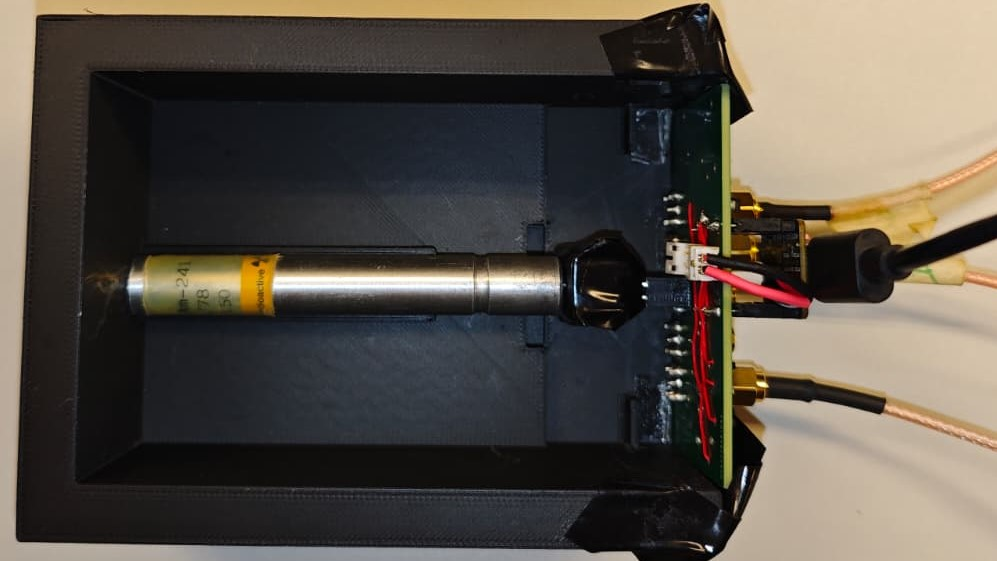
\includegraphics[width=200pt,height=127.1pt]{images/dori_case.jpg}};

% ---- 12 cm dimension (above the image, black) -------------------------
\draw [line width=1.1pt,black] (8.8,134) -- (144.4,134);
\draw [shift={(8.8,134)},rotate=0,ah,fill=black]
      (7.85,-3.78) -- (0,0) -- (7.85,3.78) -- cycle ;
\draw [shift={(144.4,134)},rotate=180,ah,fill=black]
      (7.85,-3.78) -- (0,0) -- (7.85,3.78) -- cycle ;
\node [dim,anchor=center] at (76.6,134) {12~cm};

% ---- Source holder -----------------------------------------------------
\node [anchor=south,align=center,
       text={rgb, 255:red, 204; green, 153; blue, 0 }] at (78,90) {Source Holder};
\draw [color={rgb, 255:red, 204; green, 153; blue, 0 },line width=1.1pt] (62,88) -- (58.15,79.2);
\draw [shift={(55,72)},rotate=66.4,ah,fill={rgb, 255:red, 204; green, 153; blue, 0 }]
      (7.85,-3.78) -- (0,0) -- (7.85,3.78) -- cycle ;
\draw [color={rgb, 255:red, 204; green, 153; blue, 0 },line width=1.1pt] (94,88) -- (100.4,80.5);
\draw [shift={(105.5,74.5)},rotate=130.4,ah,fill={rgb, 255:red, 204; green, 153; blue, 0 }]
      (7.85,-3.78) -- (0,0) -- (7.85,3.78) -- cycle ;

% ---- SiPM + scintillator ----------------------------------------------
\node [lbl,draw={rgb, 255:red, 26; green, 111; blue, 223 },anchor=north east]
      (sipm) at (196,112) {SiPM\\+\\Scintillator};
\draw [color={rgb, 255:red, 26; green, 111; blue, 223 },line width=1.1pt]
      (sipm.west) -| (118.1,77.4);
\draw [shift={(118.1,69.5)},rotate=90,ah,fill={rgb, 255:red, 26; green, 111; blue, 223 }]
      (7.85,-3.78) -- (0,0) -- (7.85,3.78) -- cycle ;

% ---- PCB ---------------------------------------------------------------
\node [lbl,draw={rgb, 255:red, 55; green, 173; blue, 107 },anchor=east]
      (pcb) at (196,49.9) {PCB};
\draw [color={rgb, 255:red, 55; green, 173; blue, 107 },line width=1.1pt]
      (pcb.west) -- (155.4,49.9);
\draw [shift={(147.5,49.9)},rotate=0,ah,fill={rgb, 255:red, 55; green, 173; blue, 107 }]
      (7.85,-3.78) -- (0,0) -- (7.85,3.78) -- cycle ;

% ---- 3D printed test box ----------------------------------------------
\node [lbl,draw={rgb, 255:red, 81; green, 81; blue, 81 },anchor=south east]
      (box) at (196,4) {3D Printed\\Test Box};
\draw [color={rgb, 255:red, 81; green, 81; blue, 81 },line width=1.1pt]
      (box.west) -- (131,15);
\draw [shift={(123,15)},rotate=0,ah,fill=black,
       fill={rgb, 255:red, 81; green, 81; blue, 81 }]
      (7.85,-3.78) -- (0,0) -- (7.85,3.78) -- cycle ;

\end{tikzpicture}}\\[2pt]
      \footnotesize (b)
    \end{minipage}
  \end{center}
  \smallcap{\textbf{(a)} PCB with the main functional blocks identified, together with the signal test points used for characterisation. \textbf{(b)} Assembled prototype inside the 3D printed test box, showing the sealed source holder aligned with the scintillator and SiPM.}
\end{frame}

% ---- tab:frontend ----------------------------------------------------
\begin{frame}
  \frametitle{Component Values of the Pulse Shaping Chain}
  \begin{center}
  \setlength{\tabcolsep}{10pt}
  \renewcommand{\arraystretch}{1.4}
  \begin{tabular}{c c c c c c}
    \toprule
    \multicolumn{2}{c}{\textbf{CSA}} &
    \multicolumn{2}{c}{\textbf{PZC}} &
    \multicolumn{2}{c}{\textbf{Shaper}} \\
    \cmidrule(lr){1-2}\cmidrule(lr){3-4}\cmidrule(lr){5-6}
    \textbf{Parameter} & \textbf{Value} &
    \textbf{Parameter} & \textbf{Value} &
    \textbf{Parameter} & \textbf{Value} \\
    \midrule
    \multirow{3}{*}{\shortstack{$R_f$ \\[1.6em] $C_f$}} &
    \multirow{3}{*}{\shortstack{4.7 k$\Omega$ \\[1.6em] 100 pF}} &
    $R_{\text{diff}}$ & 4.7 k$\Omega$ &
    \multirow{3}{*}{\shortstack{$R_s$ \\[1.6em] $C_s$}} &
    \multirow{3}{*}{\shortstack{10 k$\Omega$ \\[1.6em] 47 pF}} \\
    & & $R_{\text{pz}}$ & 4.7 k$\Omega$ & & \\
    & & $C_{\text{pz}}$ & 100 pF & & \\
    \midrule
    $\tau$ & 470 ns & & 470 ns & & 470 ns \\
    \bottomrule
  \end{tabular}
  \end{center}
\end{frame}

% ---- fig:shaping_chain ----------------------------------------------
\begin{frame}
  \frametitle{Transient Response of the Pulse Shaping Chain}
  \begin{center}
    \adjustbox{max width=0.72\textwidth,max height=0.6\textheight}{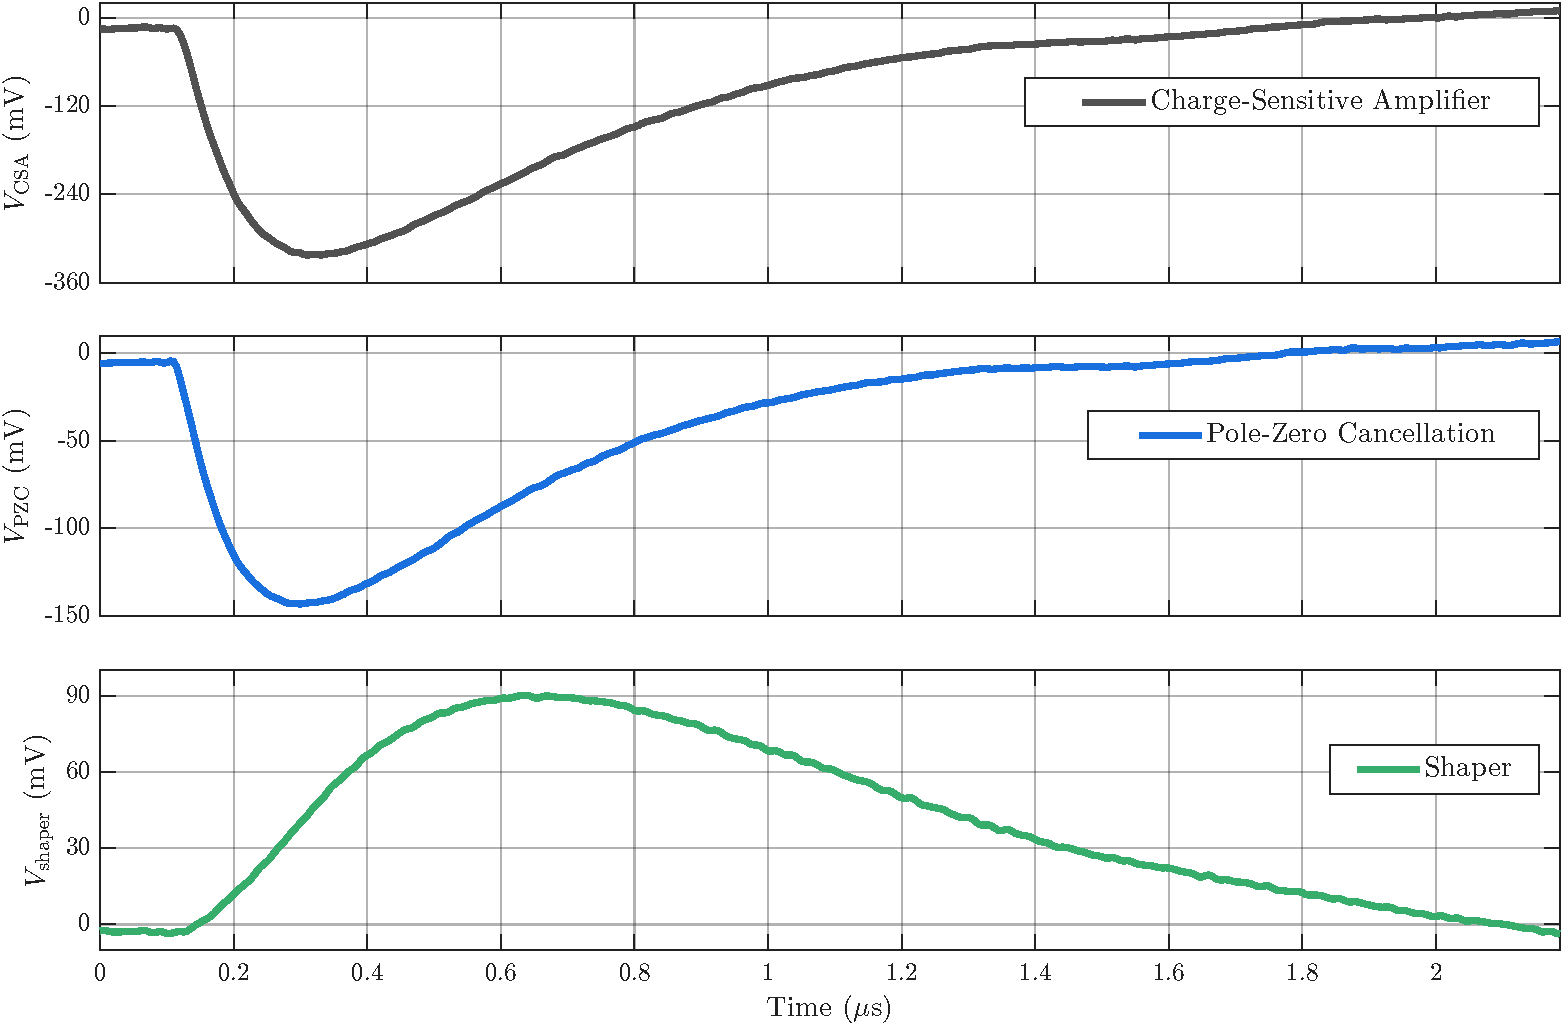
\includegraphics{images/shaping_chain_trace00001.pdf}}
  \end{center}
  \smallcap{Transient response of the CSA (grey), PZC (blue) and shaper (green) to a single $^{241}$Am event.}
\end{frame}

% ---- tab:shaping ---------------------------------------------------
\begin{frame}
  \frametitle{Timing Metrics of the Pulse Shaping Chain}
  \begin{center}
  \setlength{\tabcolsep}{14pt}
  \renewcommand{\arraystretch}{1.5}
  \begin{tabular}{l c c c}
    \toprule
     & \textbf{CSA} & \textbf{PZC} & \textbf{Shaper} \\
    \midrule
    Amplitude range (mV)            & 191--861        & 87--430         & 61--407         \\
    Peaking time (ns)               & $147 \pm 28$    & $135 \pm 25$    & $387 \pm 50$    \\
    Width at 90\% of peak (ns)      & $208 \pm 167$   & $192 \pm 141$   & $400 \pm 154$   \\
    Total shaping time ($\mu$s)     & $1.42 \pm 0.09$ & $1.26 \pm 0.07$ & $1.96 \pm 0.09$ \\
    \bottomrule
  \end{tabular}
  \end{center}
\end{frame}

% ---- fig:peak_and_hold ------------------------------------------------
\begin{frame}
  \frametitle{Peak-and-Hold Circuit}
  \begin{center}
    \adjustbox{max width=0.62\textwidth,max height=0.58\textheight}{\tikzset{every picture/.style={line width=0.75pt}}

\begin{tikzpicture}[
    x=1.5pt, y=1.5pt, yscale=-1, xscale=1,
    every node/.style={font=\normalsize, inner sep=1pt}
]

%==================== Feedback resistor R (top rail) ====================
\draw    (200,40) -- (261.9,40) ;
\draw    (261.9,40) -- (268.41,40) -- (269.86,36.39) -- (272.76,43.61) -- (275.65,36.39) -- (278.55,43.61) -- (281.45,36.39) -- (284.35,43.61) -- (287.24,36.39) -- (290.14,43.61) -- (291.59,40) -- (298.1,40) ;
\draw    (298.1,40) -- (390,40) ;

%==================== OA_1 ====================
\draw    (210,76) -- (250,100) -- (210,124) -- cycle ;
\draw    (200,90) -- (210,90) ;
\draw    (210,110) -- (192,110) ;
\draw [shift={(190,110)}, rotate=0] [line width=0.75]
       (6.56,-1.97) .. controls (4.17,-0.84) and (1.99,-0.18) .. (0,0) .. controls (1.99,0.18) and (4.17,0.84) .. (6.56,1.97) ;
\draw    (200,40) -- (200,90) ;

%==================== D_1 (feedback diode) ====================
\draw    (200,60) -- (260,60) ;
\draw    (260,60) -- (260,73.31) ;
\draw    (266.83,73.31) -- (260,86.69) -- (253.17,73.31) -- cycle ;
\draw    (253.17,86.69) -- (266.83,86.69) ;
\draw    (260,86.69) -- (260,100) ;

%==================== D_2 (output diode) ====================
\draw    (250,100) -- (273.31,100) ;
\draw    (273.31,93.17) -- (286.69,100) -- (273.31,106.83) -- cycle ;
\draw    (286.69,93.17) -- (286.69,106.83) ;
\draw    (286.69,100) -- (340,100) ;

%==================== Hold capacitor C_h ====================
\draw    (304.5,100) -- (304.5,117) ;
\draw    (300,117) -- (309,117) ;
\draw    (300,121) -- (309,121) ;
\draw    (304.5,121) -- (304.5,140) ;
\draw    (300.19,140) -- (304.5,145) -- (308.81,140) -- cycle ;

%==================== Discharge resistor R_h ====================
\draw    (330,100) -- (330,106.74) -- (333.61,108.19) -- (326.39,111.08) -- (333.61,113.98) -- (326.39,116.88) -- (333.61,119.77) -- (326.39,122.67) -- (333.61,125.57) -- (326.39,128.46) -- (330,129.91) -- (330,144) ;

%==================== Reset MOSFET ====================
\draw    (336,141) -- (336,147) ;
\draw    (336,149) -- (336,155) ;
\draw    (336,157) -- (336,163) ;
\draw    (342,140) -- (342,164) ;
\draw    (342,152) -- (355,152) ;
\draw [shift={(357,152)}, rotate=180] [line width=0.75]
       (6.56,-1.97) .. controls (4.17,-0.84) and (1.99,-0.18) .. (0,0) .. controls (1.99,0.18) and (4.17,0.84) .. (6.56,1.97) ;
\draw    (330,144) -- (336,144) ;
\draw    (336,160) -- (330,160) ;
\draw    (330,152) -- (330,166) ;
\draw    (330,152) -- (334,152) ;
\draw [shift={(336,152)}, rotate=180] [fill={rgb, 255:red, 0; green, 0; blue, 0}, fill opacity=1] [line width=0.08] [draw opacity=0]
       (3.57,-1.72) -- (0,0) -- (3.57,1.72) -- cycle ;
\draw    (325.69,166) -- (330,171) -- (334.31,166) -- cycle ;

%==================== OA_2 ====================
\draw    (340,66) -- (380,90) -- (340,114) -- cycle ;
\draw    (330,40) -- (330,80) ;
\draw    (330,80) -- (340,80) ;
\draw    (380,90) -- (408,90) ;
\draw [shift={(410,90)}, rotate=180] [line width=0.75]
       (6.56,-1.97) .. controls (4.17,-0.84) and (1.99,-0.18) .. (0,0) .. controls (1.99,0.18) and (4.17,0.84) .. (6.56,1.97) ;
\draw    (390,40) -- (390,90) ;

%==================== Junction dots ====================
\fill (200,60)    circle (0.8) ;
\fill (260,100)   circle (0.8) ;
\fill (304.5,100) circle (0.8) ;
\fill (330,100)   circle (0.8) ;
\fill (330,40)    circle (0.8) ;
\fill (330,160)   circle (0.8) ;
\fill (390,90)    circle (0.8) ;

%==================== Labels ====================
% terminals
\draw (186,110) node [anchor=east] {V$_{\mathrm{Shaper}}$};
\draw (414,90)  node [anchor=west] {V$_{\mathrm{Peak}}$};
\draw (361,152) node [anchor=west] {Reset};

% op-amps
\draw (218,100) node [anchor=west] {OA$_{1}$};
\draw (213,90)  node [anchor=west] {$-$};
\draw (213,110) node [anchor=west] {$+$};
\draw (348,90)  node [anchor=west] {OA$_{2}$};
\draw (343,80)  node [anchor=west] {$-$};
\draw (343,100) node [anchor=west] {$+$};

% passives
\draw (280,35)  node [anchor=south] {R};
\draw (250,80)  node [anchor=east]  {D$_{1}$};
\draw (280,90)  node [anchor=south] {D$_{2}$};
\draw (298,119) node [anchor=east]  {C$_{\mathrm{h}}$};
\draw (336,119) node [anchor=west]  {R$_{\mathrm{h}}$};

\end{tikzpicture}}
  \end{center}
  \smallcap{Peak-and-Hold circuit based on a precision rectifier. The outer feedback path of OA1 is shown at the top through $R$, while the local path closes through $D_1$.}
\end{frame}

% ---- fig:pulse_discrimination ------------------------------------------
\begin{frame}
  \frametitle{Transient Response of the Pulse Discrimination Chain}
  \begin{center}
    \adjustbox{max width=0.72\textwidth,max height=0.6\textheight}{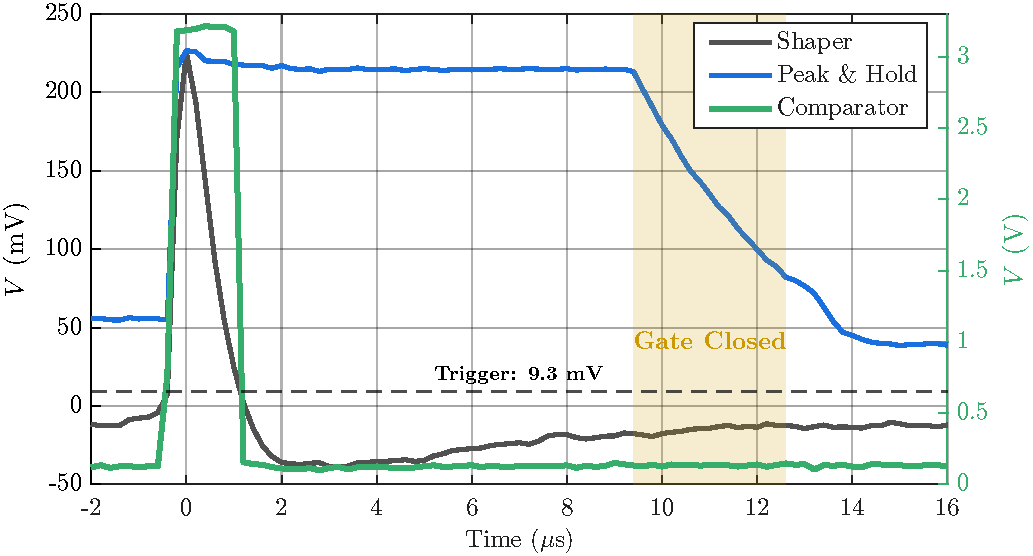
\includegraphics{images/7.5k_notitle.pdf}}
  \end{center}
  \smallcap{Transient response of the shaper (grey), comparator (green) and P\&H (blue) stages to a single $^{241}$Am event. The yellow region marks the interval during which the reset transistor is driven HIGH, allowing the hold capacitor to discharge.}
\end{frame}

% ---- tab:dead_time -----------------------------------------------------
\begin{frame}
  \frametitle{Dead Time of the Acquisition Chain}
  \begin{center}
  \setlength{\tabcolsep}{22pt}
  \renewcommand{\arraystretch}{1.3}
  \begin{tabular}{ccc}
    \toprule
    \textbf{Sampling Condition} & \textbf{Dead Time ($\mu$s)} & \textbf{Sampling Protocol} \\
    \midrule
    \textit{N/A} & 13.2 $\pm$ 0.9 & \textit{N/A} \\
    Internal MCU ADC & 59.2 $\pm$ 1.5 & Analog Read \\
    External ADC & 17.8 $\pm$ 0.4 & SPI \\
    \bottomrule
  \end{tabular}
  \end{center}
  \smallcap{Values are the mean of multiple $^{241}$Am events, with the corresponding standard deviation. With a dead time of $17.8\pm0.4$~$\mu$s, the max.\ count rate of DORI is $(56\pm1)\times10^{3}$~counts/s.}
\end{frame}

% ---- fig:validation_electronics ----------------------------------------
\begin{frame}
  \frametitle{Validation of the Front-End Electronics}
  \begin{center}
    \adjustbox{max width=0.48\textwidth,max height=0.38\textheight}{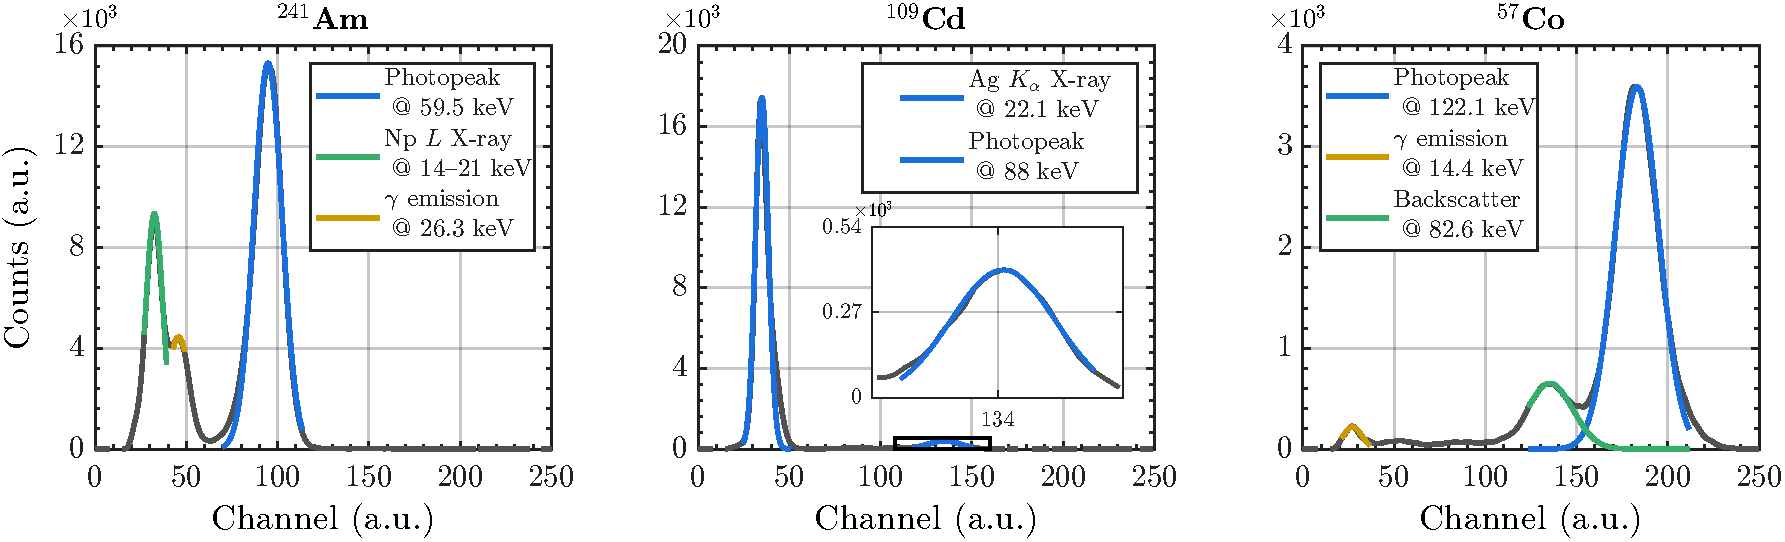
\includegraphics{images/spectra.pdf}}\\[2pt]
    \footnotesize (a)\\[3pt]
    \begin{minipage}[c]{0.44\linewidth}
      \centering
      \adjustbox{max width=\linewidth,max height=0.26\textheight}{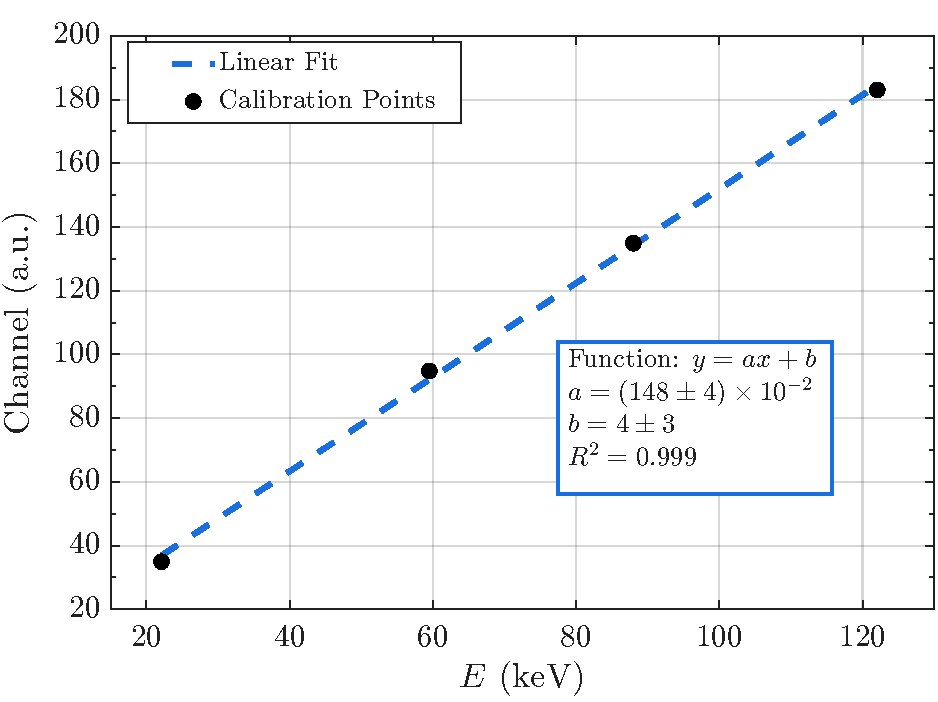
\includegraphics{images/fit_csi.pdf}}\\[2pt]
      \footnotesize (b)
    \end{minipage}%
    \hfill%
    \begin{minipage}[c]{0.44\linewidth}
      \centering
      \adjustbox{max width=\linewidth,max height=0.26\textheight}{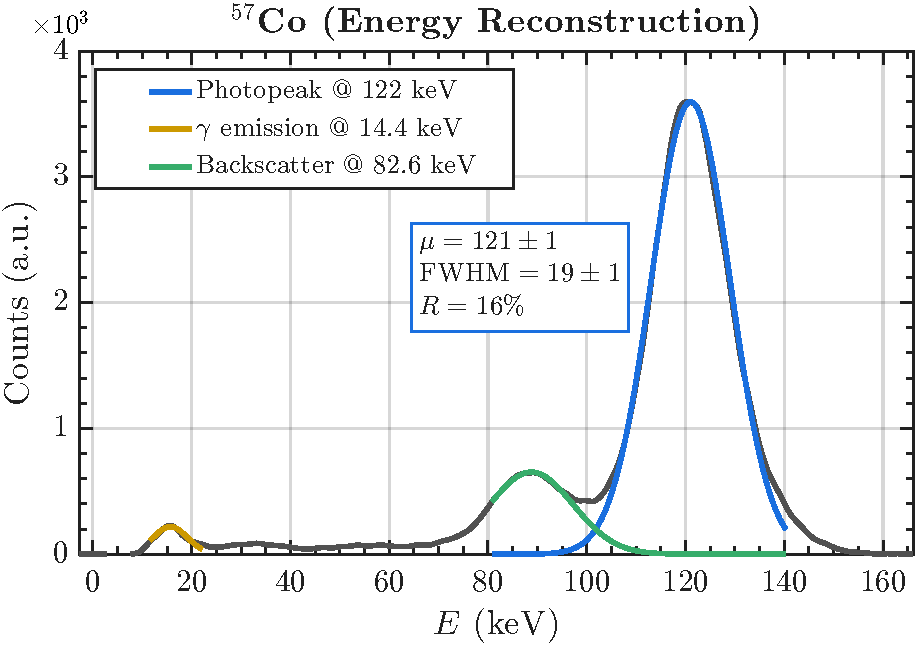
\includegraphics{images/co57_energy_reconstruction.pdf}}\\[2pt]
      \footnotesize (c)
    \end{minipage}
  \end{center}
  \smallcap{\textbf{(a)} Pulse height spectra (CsI(Tl)) for the three calibration sources. \textbf{(b)} Channel-to-energy calibration curve with linear fit. \textbf{(c)} $^{57}$Co spectrum reconstructed in energy units.}
\end{frame}

% ---- EQ-A: CsI(Tl) calibration -----------------------------------------
\begin{frame}
  \frametitle{CsI(Tl) Channel-to-Energy Calibration}
  \begin{equation*}
    C = aE + b
  \end{equation*}
  \vspace{-0.3cm}
  \begin{itemize}
    \item $C$ -- channel number, \quad $E$ -- energy in keV
    \item Fit yields $R^2 = 0.999$: linear channel-to-energy relationship confirmed up to channel 183 ($\approx$590~mV)
    \item Validation: $^{57}$Co 122~keV photopeak reconstructed at $\mu = 121 \pm 1$~keV, FWHM $19\pm1$~keV $\Rightarrow$ resolution $16\pm1\%$
    \item Confirms the front-end electronics do not introduce amplitude-dependent errors
  \end{itemize}
\end{frame}

% ======================================================================
\sectiondivider{Chapter 3\\[4pt]\Large Calibration of the DORI Prototype}

% ---- fig:bremss_calibration -------------------------------------------
\begin{frame}
  \frametitle{Bremsstrahlung Spectra}
  \begin{center}
    \begin{minipage}[c]{0.48\linewidth}
      \centering
      \adjustbox{max width=\linewidth,max height=0.6\textheight}{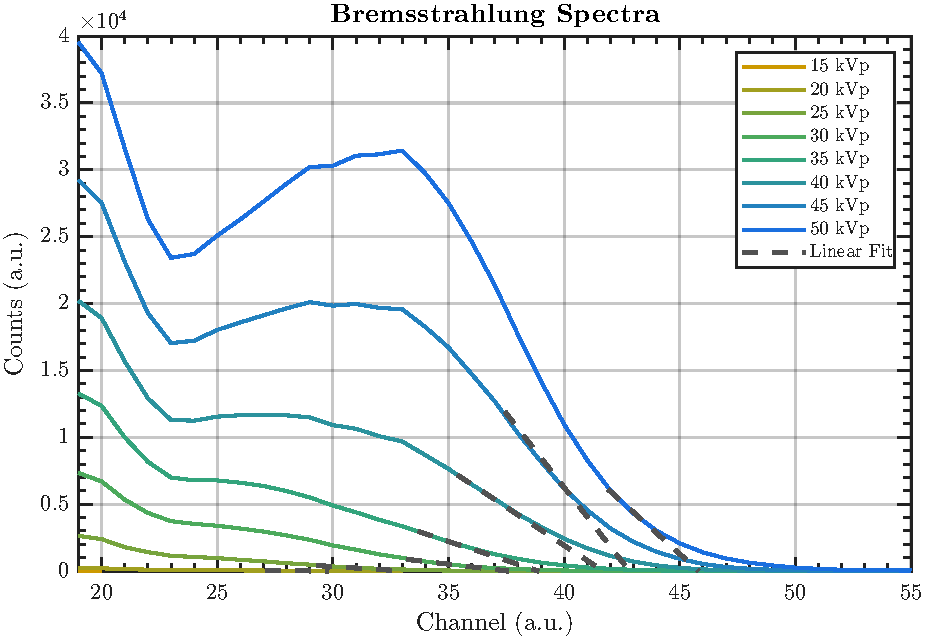
\includegraphics{images/bremsstrahlung_fits.pdf}}\\[2pt]
      \footnotesize (a)
    \end{minipage}%
    \hfill%
    \begin{minipage}[c]{0.48\linewidth}
      \centering
      \adjustbox{max width=\linewidth,max height=0.6\textheight}{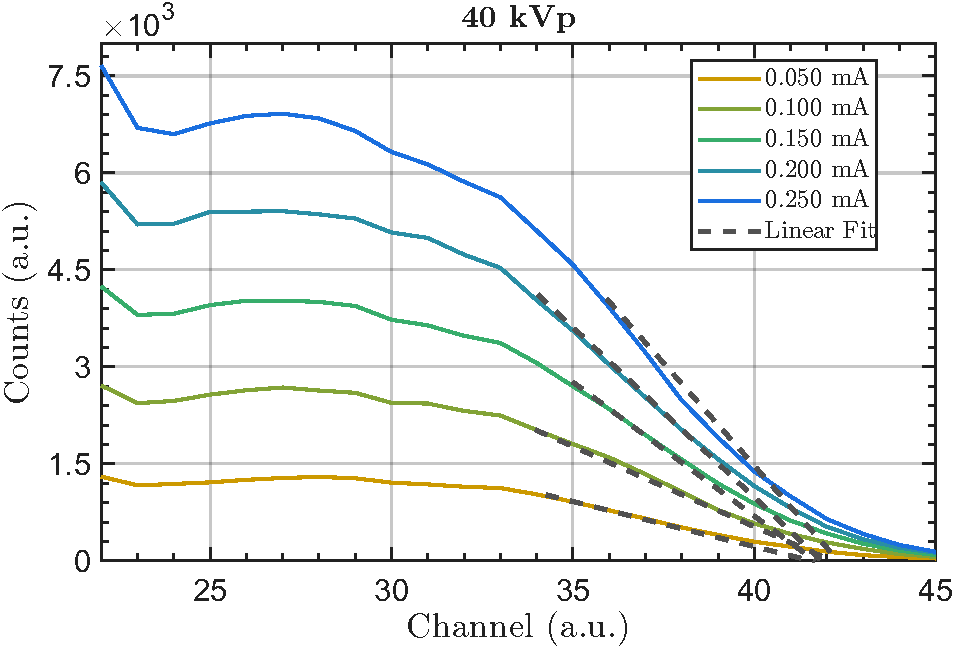
\includegraphics{images/bremsstrahlung_40kVp_vs_current.pdf}}\\[2pt]
      \footnotesize (b)
    \end{minipage}
  \end{center}
  \smallcap{Background subtracted; \textbf{(a)} acquired at 0.250~mA for tube voltages 15--50~kVp; \textbf{(b)} acquired at 40~kVp for tube currents 0.050--0.250~mA.}
\end{frame}

% ---- tab:endpoints -------------------------------------------------
\begin{frame}
  \frametitle{Bremsstrahlung Endpoint Channel per Tube Voltage}
  \begin{center}
  \small
  \begin{tabular}{>{\centering\arraybackslash}m{0.16\textwidth}
                  >{\centering\arraybackslash}m{0.09\textwidth}
                  >{\centering\arraybackslash}m{0.09\textwidth}
                  >{\centering\arraybackslash}m{0.09\textwidth}
                  >{\centering\arraybackslash}m{0.09\textwidth}
                  >{\centering\arraybackslash}m{0.09\textwidth}
                  >{\centering\arraybackslash}m{0.09\textwidth}}
    \toprule
    \textbf{Tube Voltage (kVp)} & \textbf{20} & \textbf{25} & \textbf{30} & \textbf{35} & \textbf{40} & \textbf{45} \\
    \midrule
    \textbf{Endpoint Ch. (a.u.)}
    & $31 \pm 3\%$ & $33 \pm 3\%$ & $37 \pm 1\%$ & $39 \pm 1\%$ & $42 \pm 1\%$ & $43 \pm 1\%$ \\
    \bottomrule
  \end{tabular}\\[6pt]
  \begin{tabular}{>{\centering\arraybackslash}m{0.16\textwidth}>{\centering\arraybackslash}m{0.09\textwidth}}
    \toprule
    \textbf{50} \\
    \midrule
    $45 \pm 2\%$ \\
    \bottomrule
  \end{tabular}
  \end{center}
  \smallcap{Values are the mean of five acquisitions with the maximum deviation from the mean.}
\end{frame}

% ---- fig:source_spectra --------------------------------------------
\begin{frame}
  \frametitle{Reference Source Spectra}
  \begin{center}
    \begin{minipage}[c]{0.48\linewidth}
      \centering
      \adjustbox{max width=\linewidth,max height=0.6\textheight}{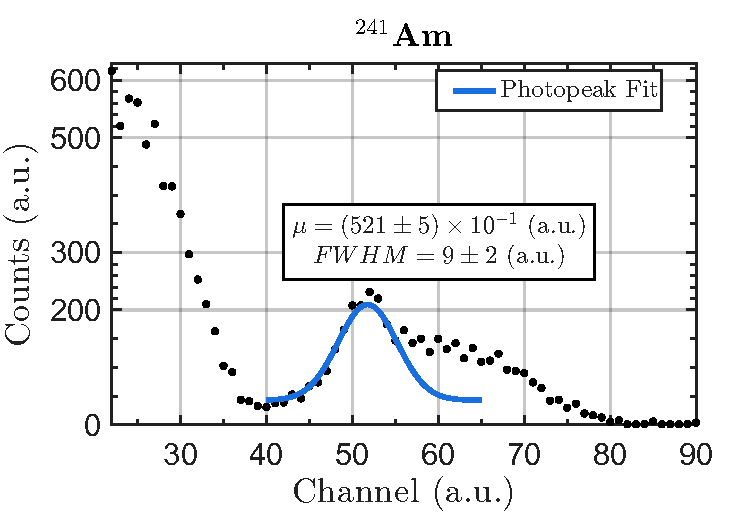
\includegraphics{images/plastic_Am-241.pdf}}\\[2pt]
      \footnotesize (a)
    \end{minipage}%
    \hfill%
    \begin{minipage}[c]{0.48\linewidth}
      \centering
      \adjustbox{max width=\linewidth,max height=0.6\textheight}{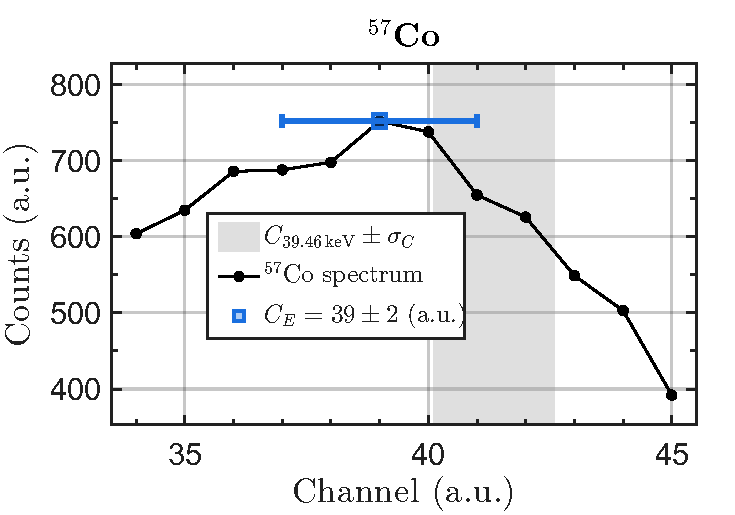
\includegraphics{images/plastic_Co-57_fit.pdf}}\\[2pt]
      \footnotesize (b)
    \end{minipage}
  \end{center}
  \smallcap{Background subtracted, plastic scintillator. \textbf{(a)} $^{241}$Am, Gaussian fit to the 59.5~keV photopeak. \textbf{(b)} $^{57}$Co Compton Edge at 39.46~keV.}
\end{frame}

% ---- fig:energy_calibration ------------------------------------------
\begin{frame}
  \frametitle{Energy Calibration of the DORI Prototype}
  \begin{center}
    \adjustbox{max width=0.6\textwidth,max height=0.6\textheight}{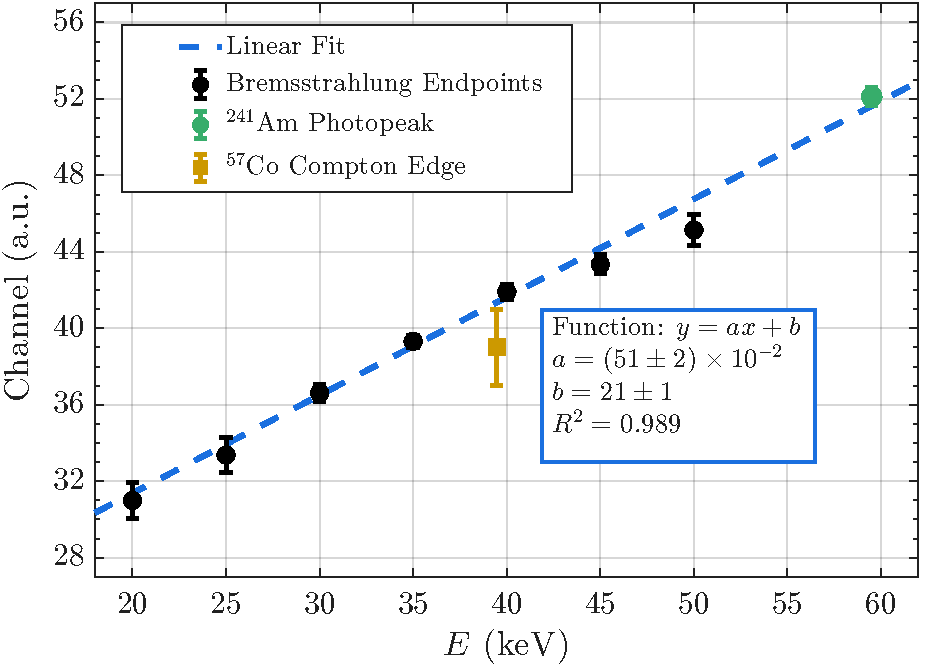
\includegraphics{images/energy.pdf}}
  \end{center}
  \smallcap{Weighted least-squares energy calibration, obtained from the seven \emph{Bremsstrahlung} endpoints and the $^{241}$Am photopeak centroid. The $^{57}$Co Compton edge is superimposed for validation.}
\end{frame}

% ---- EQ-B: energy calibration formula --------------------------------
\begin{frame}
  \frametitle{DORI Energy Calibration Formula}
  \begin{equation*}
    C = aE + b, \qquad R^2 = 0.989 \ \ (\text{20--60 keV})
  \end{equation*}
  \begin{equation*}
    E = \frac{C - 21}{0.51}
  \end{equation*}
  \begin{equation*}
    \sigma_E = \frac{1}{0.51}\sqrt{(0.02)^2\,E^2 + 1^2}
  \end{equation*}
  \vspace{-0.2cm}
  \begin{itemize}
    \item $^{241}$Am centroid $\Rightarrow$ energy resolution $R = (29\pm5)\%$ at 59.5~keV
    \item Calibrated interval: 20 to 60~keV (locally linear response)
  \end{itemize}
\end{frame}

% ---- tab:nseries ----------------------------------------------------
\begin{frame}
  \frametitle{N-Series Radiation Qualities}
  \begin{center}
  \begin{tabular}{cccc}
    \toprule
    \textbf{\begin{tabular}[b]{@{}c@{}}Radiation\\Quality\end{tabular}} &
    \textbf{\begin{tabular}[b]{@{}c@{}}Tube Potential\\(kVp)\end{tabular}} &
    \textbf{\begin{tabular}[b]{@{}c@{}}Added\\Filtration\end{tabular}} &
    \begin{tabular}[b]{@{}c@{}}$\bm{h_{pK}(10)}$\\\textbf{(Sv/Gy)}\end{tabular} \\
    \midrule
    \textbf{N-25} & 25 & 2 mm Al & 0.574 \\
    \textbf{N-30} & 30 & 4 mm Al & 0.815 \\
    \textbf{N-40} & 40 & 4 mm Al + 0.21 mm Cu & 1.210 \\
    \bottomrule
  \end{tabular}
  \end{center}
  \smallcap{Coefficients correspond to the ISO slab phantom at 1-meter normal incidence (ISO~4037 series).}
\end{frame}

% ---- fig:setup --------------------------------------------------------
\begin{frame}
  \frametitle{Dose Calibration Setup}
  \begin{center}
    \adjustbox{max width=0.6\textwidth,max height=0.6\textheight}{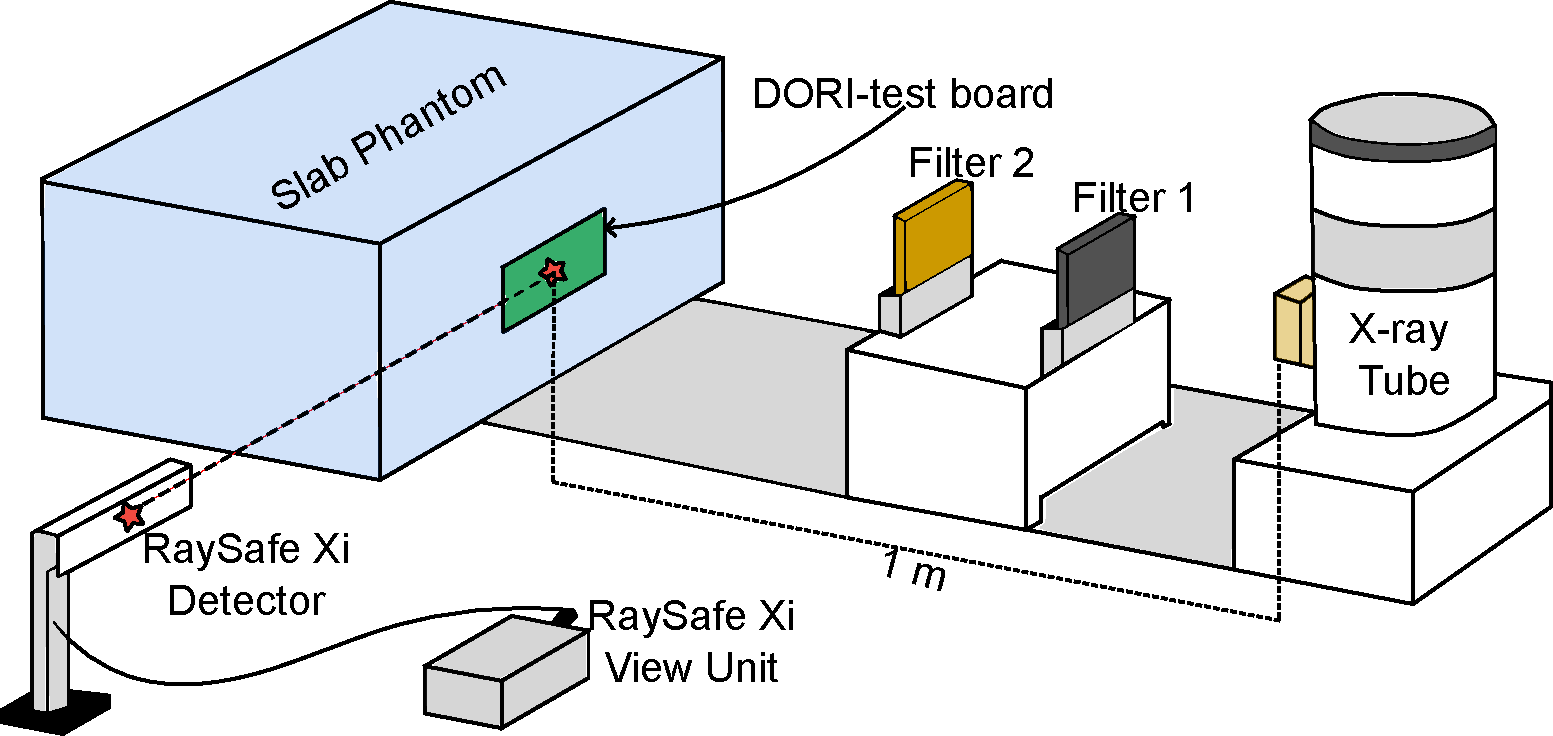
\includegraphics{images/dose.pdf}}
  \end{center}
  \smallcap{The DORI-test board is placed at the reference measurement point (red star), against the front wall of the built slab phantom. The RaySafe Xi detector is positioned at the same point free-in-air, phantom removed.}
\end{frame}

% ---- fig:dose ----------------------------------------------------------
\begin{frame}
  \frametitle{ISO 4037 N-Series Spectra \& Reference Rate}
  \begin{center}
    \begin{minipage}[c]{0.48\linewidth}
      \centering
      \adjustbox{max width=\linewidth,max height=0.6\textheight}{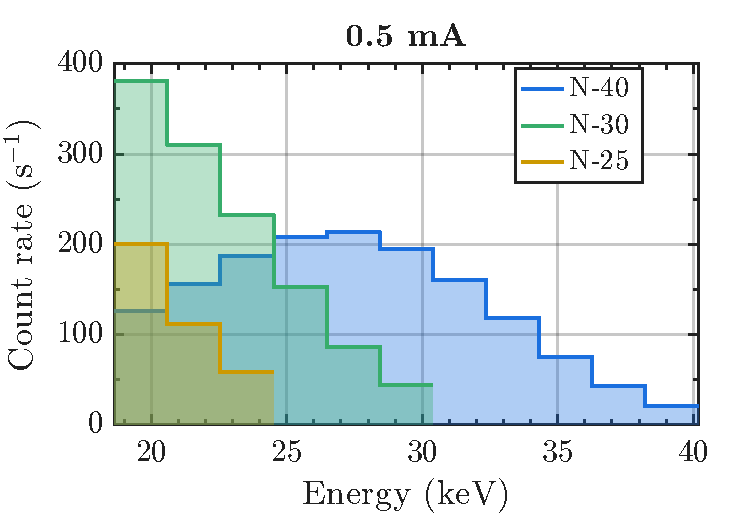
\includegraphics{images/fig1_spectra.pdf}}\\[2pt]
      \footnotesize (a)
    \end{minipage}%
    \hfill%
    \begin{minipage}[c]{0.48\linewidth}
      \centering
      \adjustbox{max width=\linewidth,max height=0.6\textheight}{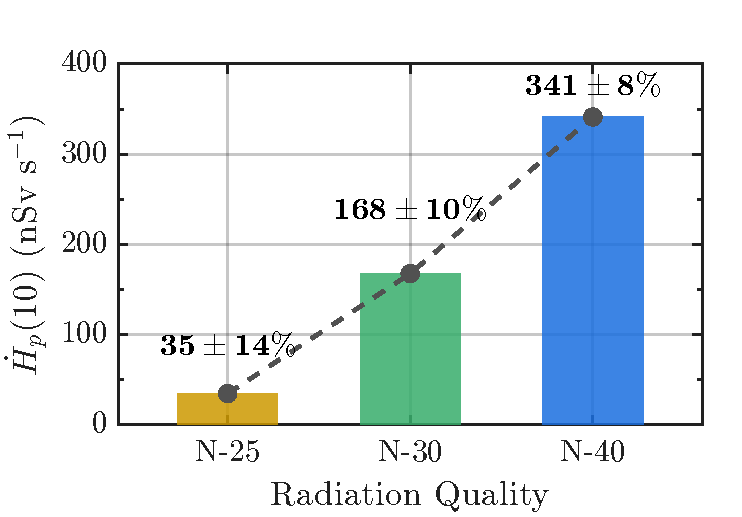
\includegraphics{images/fig2_reference.pdf}}\\[2pt]
      \footnotesize (b)
    \end{minipage}
  \end{center}
  \smallcap{N-25, N-30 and N-40, acquired at 0.500~mA for 2 minutes. \textbf{(a)} Energy spectra. \textbf{(b)} Reference $\dot{H}_p(10)$.}
\end{frame}

% ---- fig:scan (+ maxdev eq) --------------------------------------------
\begin{frame}
  \frametitle{Bin-Boundary Optimisation}
  \begin{columns}[T]
    \begin{column}{0.55\textwidth}
      \adjustbox{max width=\linewidth,max height=0.62\textheight}{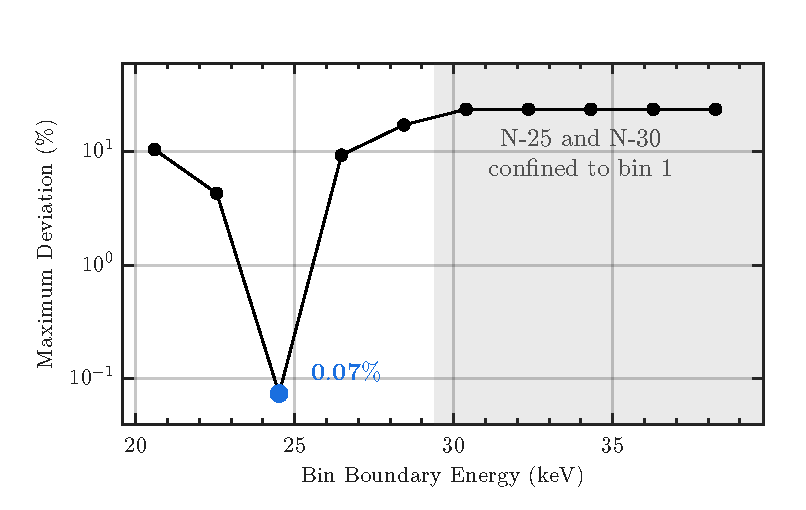
\includegraphics{images/fig6_boundary_scan.pdf}}
    \end{column}
    \begin{column}{0.45\textwidth}
      \begin{equation*}
        \delta_{\max} = \max_{q} \left| \frac{H_p(10)_q^{\,\mathrm{calc}}}{H_p(10)_q^{\,\mathrm{ref}}} - 1 \right| \times 100\%
      \end{equation*}
      \footnotesize
      Minimum $\delta_{\max} = 0.07\%$ at a boundary of 24.5~keV. Bins adopted: $N_1 \in [20,25]$~keV, $N_2 \in \,]25,40]$~keV.
    \end{column}
  \end{columns}
\end{frame}

% ---- tab:matrix -----------------------------------------------------
\begin{frame}
  \frametitle{Count Rates per Bin \& Reference $\dot{H}_p(10)$}
  \begin{center}
  \begin{tabular}{cccc}
    \toprule
    \textbf{\begin{tabular}[b]{@{}c@{}}Radiation\\Quality\end{tabular}} &
    \textbf{\begin{tabular}[b]{@{}c@{}}$\bm{{N}_1}$\\(s$^{-1}$)\end{tabular}} &
    \textbf{\begin{tabular}[b]{@{}c@{}}$\bm{{N}_2}$\\(s$^{-1}$)\end{tabular}} &
    \textbf{\begin{tabular}[b]{@{}c@{}}$\bm{\dot{H}_p(10)}$\\(nSv s$^{-1}$)\end{tabular}} \\
    \midrule
    \textbf{N-25} &  370 &    0 & $35 \pm 5$  \\
    \textbf{N-30} &  923 &  283 & $168 \pm 16$ \\
    \textbf{N-40} &  469 & 1033 & $341 \pm 26$ \\
    \bottomrule
  \end{tabular}
  \end{center}
\end{frame}

% ---- EQ-D: dose calibration weights -----------------------------------
\begin{frame}
  \frametitle{Dose Calibration Weights \& Formula}
  \begin{equation*}
    w_1 = 93.4 \pm 18.4, \qquad w_2 = 287.9 \pm 29.3\ \left[\tfrac{\mathrm{pSv}}{\mathrm{count}}\right]
  \end{equation*}
  \begin{equation*}
    H_p(10) = 93.4\,N_1 + 287.9\,N_2
  \end{equation*}
  \begin{equation*}
    \sigma_{H_p(10)} = \sqrt{\left(18.4\,N_1\right)^2 + \left(29.3\,N_2\right)^2}
  \end{equation*}
  \vspace{-0.2cm}
  \footnotesize
  A count in the upper bin carries $3.1\times$ the dose of a count in the lower bin.
\end{frame}

% ---- fig:dose_calibration ----------------------------------------------
\begin{frame}
  \frametitle{Fit Residuals \& Leave-One-Out Deviations}
  \begin{center}
    \adjustbox{max width=0.6\textwidth,max height=0.6\textheight}{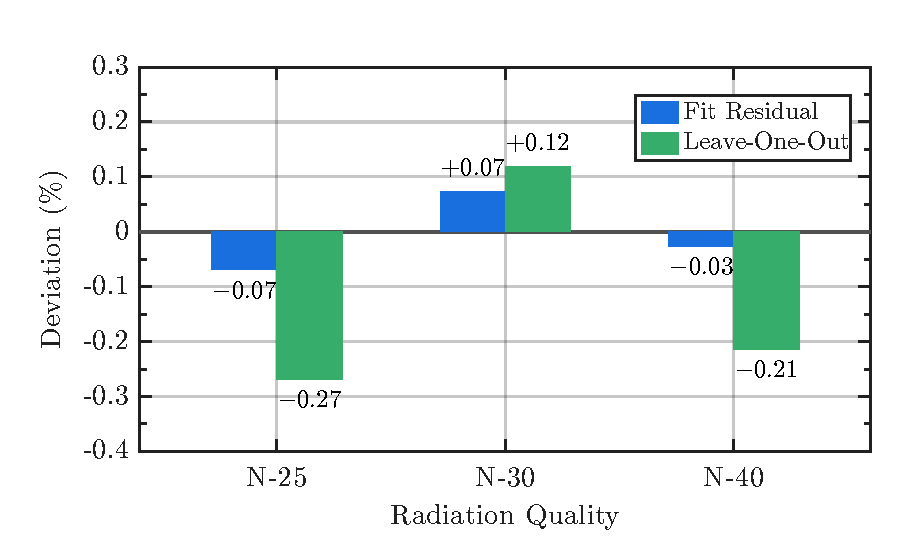
\includegraphics{images/dose_calibration.pdf}}
  \end{center}
  \smallcap{Deviation of the reconstructed $\dot{H}_p(10)$ from the reference value, per radiation quality. Blue bars: fit residuals. Green bars: leave-one-out predictions.}
\end{frame}

% ---- fig:dose_linearity -----------------------------------------------
\begin{frame}
  \frametitle{Reconstructed $\dot{H}_p(10)$ vs Tube Current}
  \begin{center}
    \adjustbox{max width=0.7\textwidth,max height=0.6\textheight}{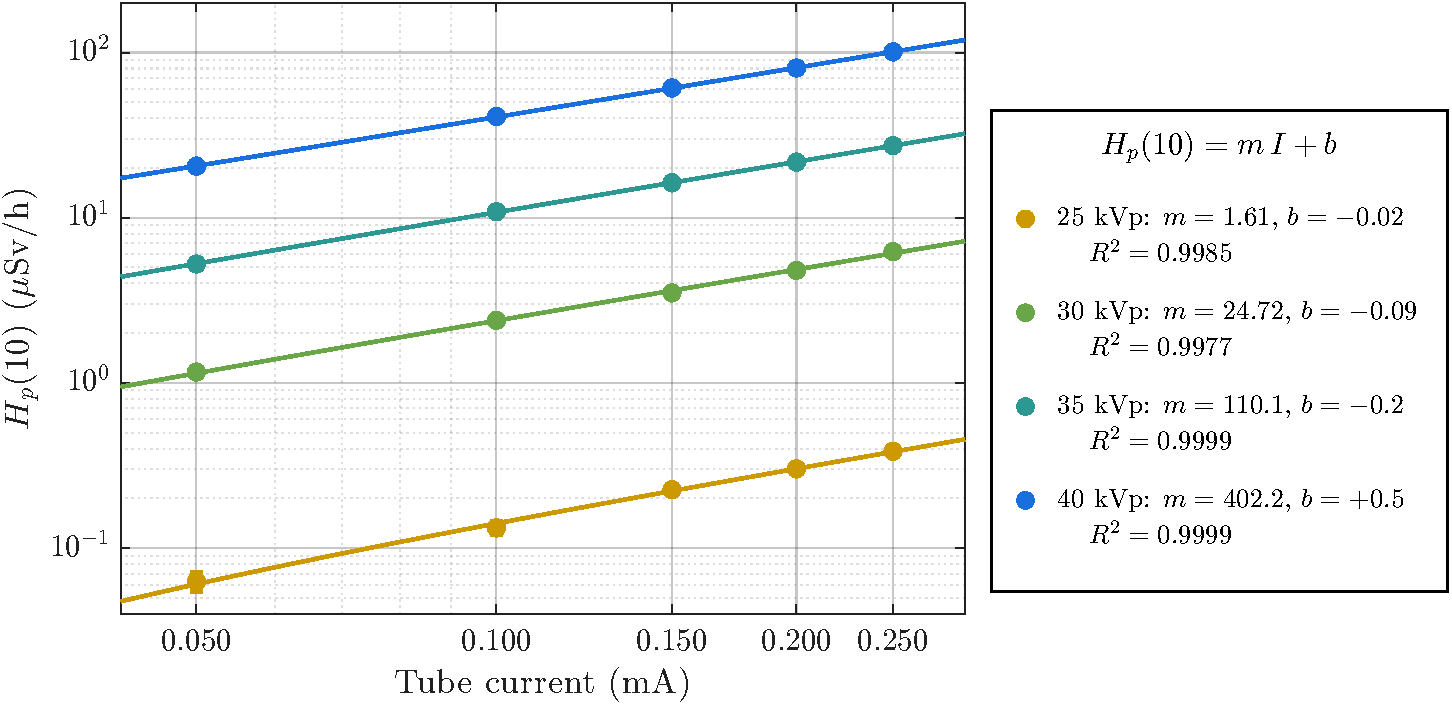
\includegraphics{images/dose_rate_linearity.pdf}}
  \end{center}
  \smallcap{Tube potentials 25--40~kVp, currents 0.050--0.250~mA. Dose rate increases linearly with tube current at every potential ($R^2 \geq 0.998$).}
\end{frame}

% ======================================================================
\sectiondivider{Chapter 4\\[4pt]\Large Final Prototype}

% ---- fig:prototype -------------------------------------------------
\begin{frame}
  \frametitle{Final DORI Prototype}
  \begin{center}
    \adjustbox{max width=0.9\textwidth,max height=0.58\textheight}{\begin{tikzpicture}[x=1pt,y=1pt,
    every node/.style={font=\footnotesize},
    ah/.style={draw opacity=0,line width=0.08,fill opacity=1},
    ahs/.style={ah,scale=0.55},
    lbl/.style={fill=white,align=center,inner sep=2.5pt,line width=0.6pt},
    dim/.style={fill=white,align=center,inner sep=2pt,draw=none,font=\scriptsize},
    pan/.style={font=\footnotesize\bfseries,inner sep=0pt,anchor=north}]

% =========================================================================
% (a)  bottom shell  --  image x: 59.5 -> 237.25 , y: 172 -> 308.9
% =========================================================================
\node [anchor=south west,inner sep=0] at (59.5,172)
  {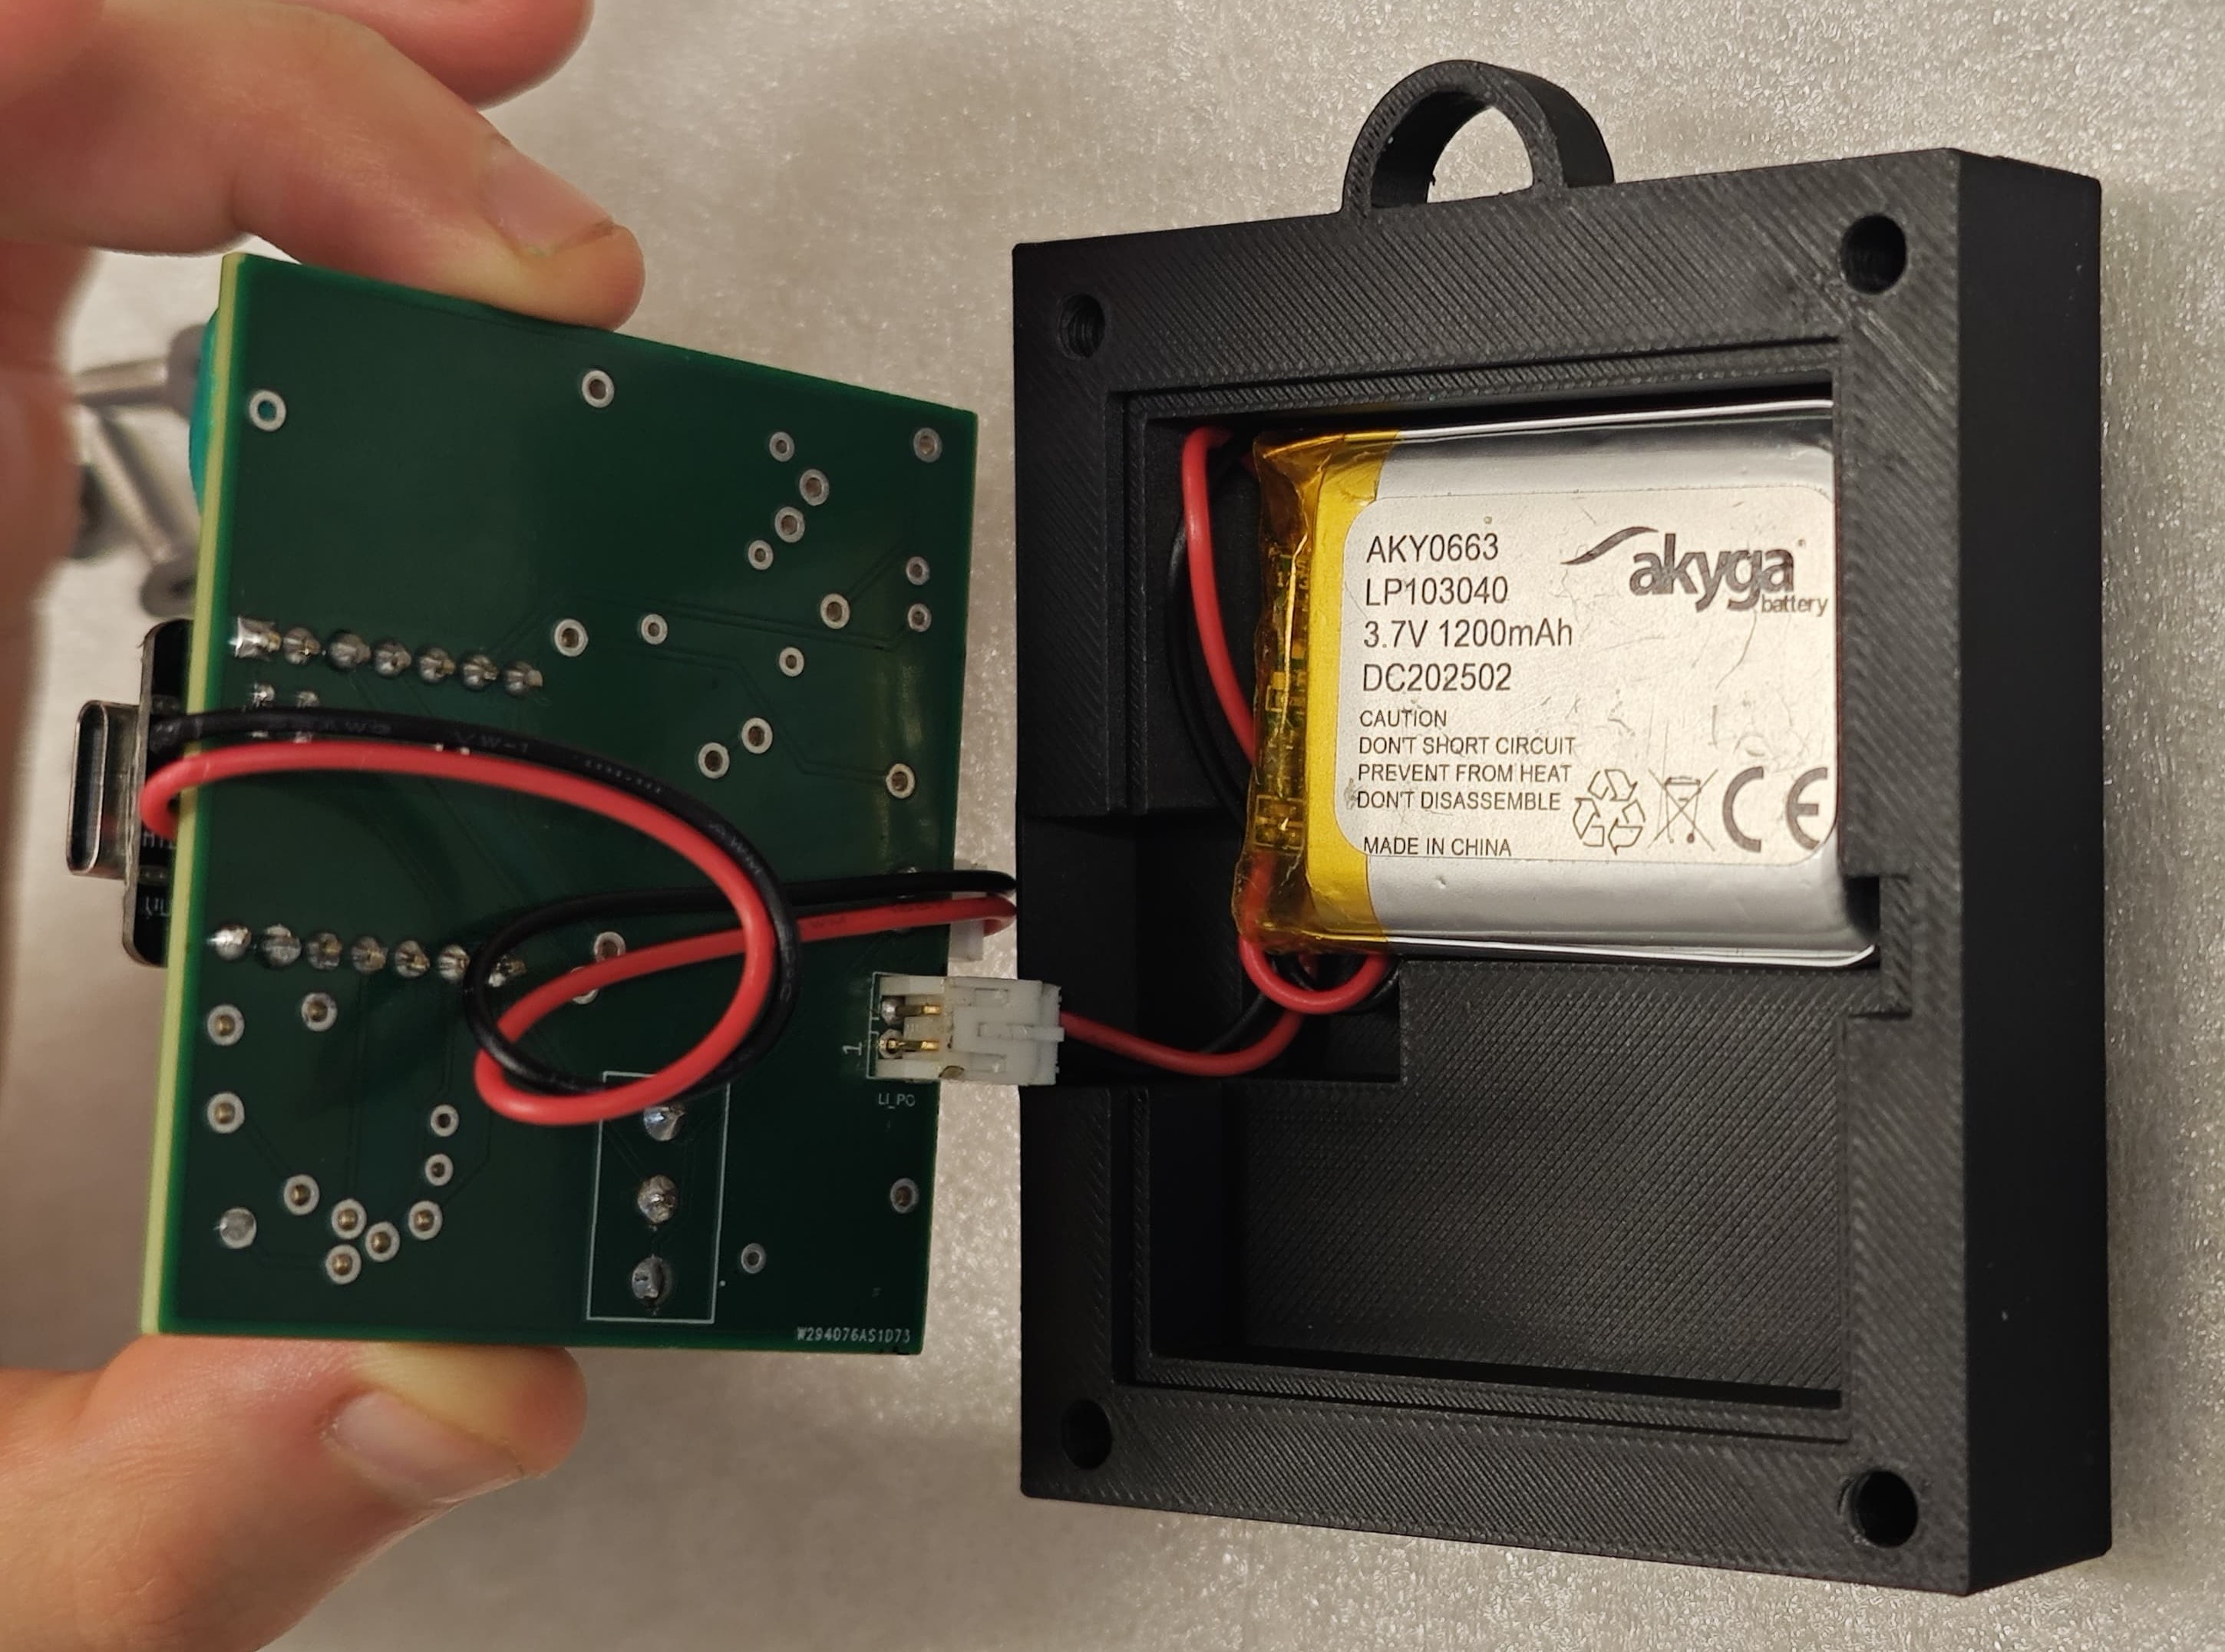
\includegraphics[width=177.75pt,height=136.9pt]{images/baixo.jpg}};

% ---- Battery + cables compartment ---------------------------------------
\node [lbl,draw={rgb, 255:red, 81; green, 81; blue, 81 },anchor=center]
      (batt) at (106.1,280.6) {Battery + Cables\\Compartment};
\draw [color={rgb, 255:red, 81; green, 81; blue, 81 },line width=1.1pt]
      ([xshift=12.5pt]batt.south) -- (147.0,240.4);
\draw [shift={(152.6,234.7)},rotate=134.3,ah,
       fill={rgb, 255:red, 81; green, 81; blue, 81 }]
      (7.85,-3.78) -- (0,0) -- (7.85,3.78) -- cycle ;

% ---- Power cables -------------------------------------------------------
\node [lbl,draw={rgb, 255:red, 241; green, 74; blue, 64 },anchor=center]
      (pcab) at (163.25,189.1) {Power\\Cables};
\draw [color={rgb, 255:red, 241; green, 74; blue, 64 },line width=1.1pt]
      ([xshift=-8pt]pcab.north) -- (151.0,213.7);
\draw [shift={(148.6,221.35)},rotate=287.4,ah,
       fill={rgb, 255:red, 241; green, 74; blue, 64 }]
      (7.85,-3.78) -- (0,0) -- (7.85,3.78) -- cycle ;
\draw [color={rgb, 255:red, 241; green, 74; blue, 64 },line width=1.1pt]
      ([xshift=-8pt]pcab.north) -- (126.4,217.7);
\draw [shift={(119.6,221.85)},rotate=328.6,ah,
       fill={rgb, 255:red, 241; green, 74; blue, 64 }]
      (7.85,-3.78) -- (0,0) -- (7.85,3.78) -- cycle ;

% ---- Panel letter (centred on the image) --------------------------------
\node [pan] at (148.375,164) {(a)};
\begin{scope}[yshift=8pt]
% =========================================================================
% (b)  middle shell  --  image x: 0 -> 135.7 , y: 0 -> 146
% =========================================================================
\node [anchor=south west,inner sep=0] at (0,0)
  {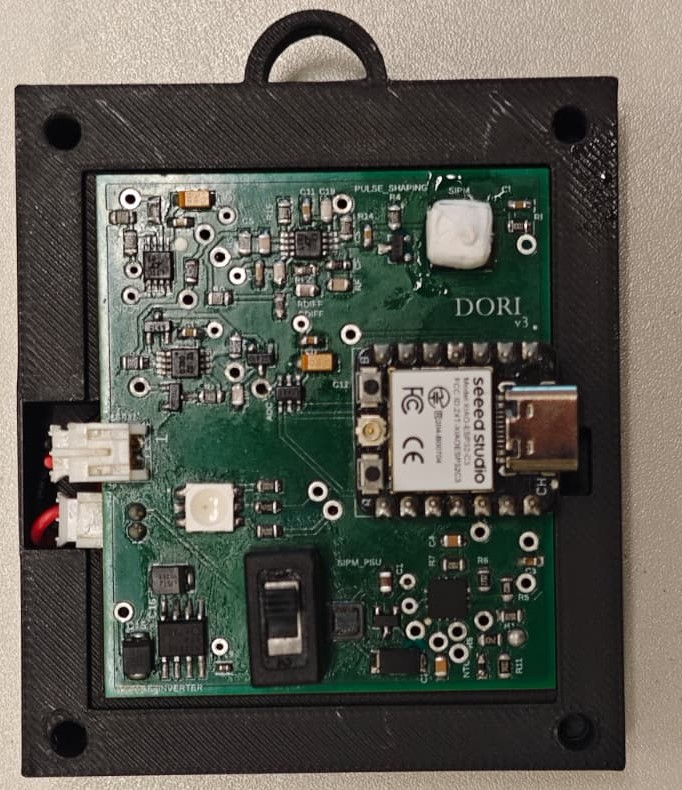
\includegraphics[width=135.7pt,height=146pt]{images/meio.jpg}};

% ---- Teflon-wrapped scintillator ---------------------------------------
\node [lbl,draw={rgb, 255:red, 26; green, 111; blue, 223 },anchor=center]
      (tefl) at (56.65,126.2) {Teflon-wrapped\\Scintillator};
\draw [color={rgb, 255:red, 26; green, 111; blue, 223 },line width=1.1pt]
      ([xshift=9.35pt]tefl.south) -- (79.2,107.0);
\draw [shift={(86.0,102.8)},rotate=148.2,ah,
       fill={rgb, 255:red, 26; green, 111; blue, 223 }]
      (7.85,-3.78) -- (0,0) -- (7.85,3.78) -- cycle ;

% ---- Width dimension (6.3 cm) ------------------------------------------
\draw [line width=1.1pt,black] (2,-4) -- (123.5,-4);
\draw [shift={(2,-4)},rotate=0,ah,fill=black]
      (7.85,-3.78) -- (0,0) -- (7.85,3.78) -- cycle ;
\draw [shift={(123.5,-4)},rotate=180,ah,fill=black]
      (7.85,-3.78) -- (0,0) -- (7.85,3.78) -- cycle ;
\node [dim,anchor=center] at (62.8,-4) {6.3~cm};
% ---- Height dimension (7.2 cm) -----------------------------------------
\draw [line width=1.1pt,black] (-4,3.5) -- (-4,132.5);
\draw [shift={(-4,3.5)},rotate=90,ah,fill=black]
      (7.85,-3.78) -- (0,0) -- (7.85,3.78) -- cycle ;
\draw [shift={(-4,132.5)},rotate=270,ah,fill=black]
      (7.85,-3.78) -- (0,0) -- (7.85,3.78) -- cycle ;
\node [dim,anchor=center,rotate=90] at (-4,68) {7.2~cm};

% ---- Panel letter -------------------------------------------------------
\node [pan] at (67.85,-10) {(b)};

% =========================================================================
% (c)  top shell  --  image x: 159.7 -> 296.8 , y: 0 -> 146
% =========================================================================
\node [anchor=south west,inner sep=0] at (159.7,0)
  {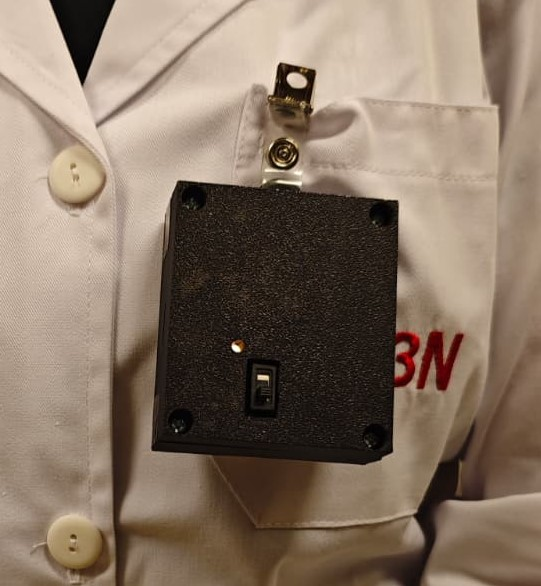
\includegraphics[width=137.1pt,height=146pt]{images/cima.jpg}};
% ---- LED --------------------------------------------------------------
\node [lbl,draw={rgb, 255:red, 204; green, 153; blue, 0 },anchor=center]
      (led) at (181.75,71.45) {LED On};
\draw [color={rgb, 255:red, 204; green, 153; blue, 0 },line width=1.1pt]
      (led.east) -- (217.6,61.6);
\draw [shift={(219.5,60.4)},rotate=151.2,ah,
       fill={rgb, 255:red, 204; green, 153; blue, 0 }]
      (7.85,-3.78) -- (0,0) -- (7.85,3.78) -- cycle ;
% ---- Badge clip ---------------------------------------------------------
\node [lbl,draw={rgb, 255:red, 55; green, 173; blue, 107 },anchor=center]
      (badge) at (269.4,107.7) {Badge Clip};
\draw [color={rgb, 255:red, 55; green, 173; blue, 107 },line width=1.1pt]
      (badge.north) -- (245.3,120.7);
\draw [shift={(237.5,122.6)},rotate=346.6,ah,
       fill={rgb, 255:red, 55; green, 173; blue, 107 }]
      (7.85,-3.78) -- (0,0) -- (7.85,3.78) -- cycle ;


% ---- Power switch -------------------------------------------------------
\node [lbl,draw={rgb, 255:red, 241; green, 74; blue, 64 },anchor=center]
      (psw) at (265.15,47) {Power\\Switch};
\draw [color={rgb, 255:red, 241; green, 74; blue, 64 },line width=1.1pt]
      (psw.west) -- (240,47);
\draw [shift={(232,47)},rotate=0,ah,
       fill={rgb, 255:red, 241; green, 74; blue, 64 }]
      (7.85,-3.78) -- (0,0) -- (7.85,3.78) -- cycle ;

% ---- Thickness dimension (2.5 cm, short arrow -> scaled heads) ----------
\draw [line width=1.1pt,black] (201.0,92.9) -- (205.8,101.6);
\draw [shift={(201.0,92.9)},rotate=61.1,ahs,fill=black]
      (7.85,-3.78) -- (0,0) -- (7.85,3.78) -- cycle ;
\draw [shift={(205.8,101.6)},rotate=241.1,ahs,fill=black]
      (7.85,-3.78) -- (0,0) -- (7.85,3.78) -- cycle ;
\node [dim,anchor=center,rotate=61] at (194.7,102.2) {2.5~cm};
% ---- Panel letter -------------------------------------------------------
\node [pan] at (228.25,-10) {(c)};
\end{scope}
\end{tikzpicture}}
  \end{center}
  \smallcap{\textbf{(a)} Bottom layer of the enclosure with the LiPo battery compartment. \textbf{(b)} Assembled PCB with the Teflon-wrapped scintillator coupled to the SiPM. \textbf{(c)} Closed prototype worn over a lab coat, with badge clip, power switch and LED.}
\end{frame}

% ---- tab:endpoints_prototype ---------------------------------------
\begin{frame}
  \frametitle{Endpoint Channel --- Final Prototype}
  \begin{center}
  \small
  \begin{tabularx}{0.9\textwidth}{>{\centering\arraybackslash}m{0.18\textwidth}
                               *{6}{>{\centering\arraybackslash}X}}
    \toprule
    \textbf{Tube Voltage (kVp)} & \textbf{25} & \textbf{30} & \textbf{35} & \textbf{40} & \textbf{45} & \textbf{50} \\
    \midrule
    \textbf{Endpoint Ch. (a.u.)}
    & $30 \pm 4\%$
    & $34 \pm 1\%$
    & $36 \pm 1\%$
    & $39 \pm 1\%$
    & $41 \pm 1\%$
    & $42 \pm 2\%$ \\
    \bottomrule
  \end{tabularx}
  \end{center}
  \smallcap{Values are the mean of three acquisitions with the maximum deviation from the mean.}
\end{frame}

% ---- fig:channel_response ----------------------------------------------
\begin{frame}
  \frametitle{Endpoint Correspondence: Test Board vs Final Prototype}
  \begin{center}
    \adjustbox{max width=0.6\textwidth,max height=0.6\textheight}{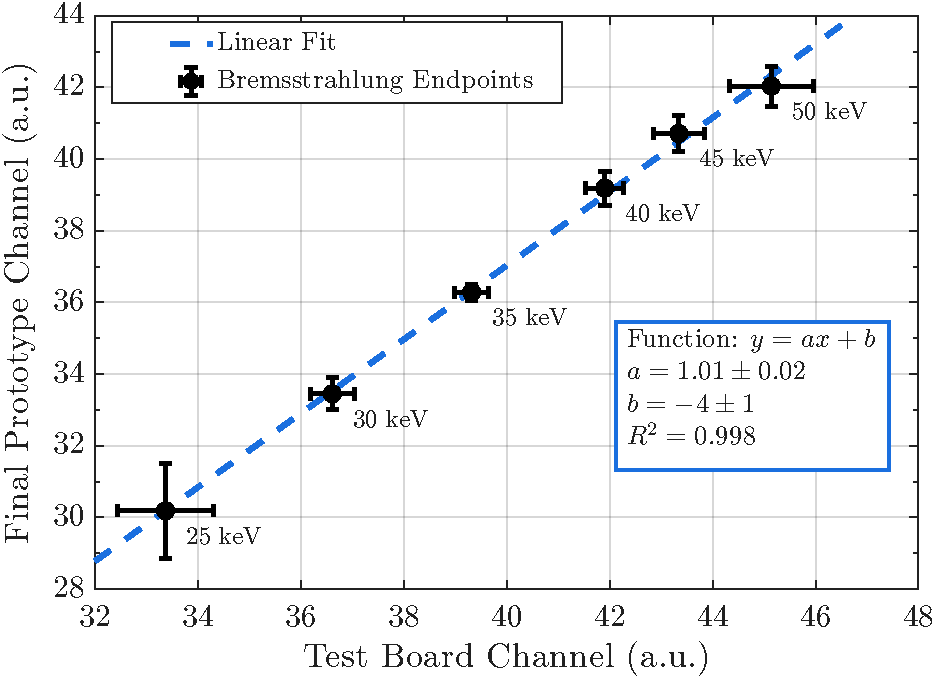
\includegraphics{images/channel_transfer.pdf}}
  \end{center}
  \smallcap{Linear fit, $R^2=0.998$, slope $1.01\pm0.02$: gain preserved. Final prototype records events $3.0\pm0.2$ channels below the test board (baseline shift $\approx$9.6~mV); the energy calibration slope carries over, with only the intercept displaced.}
\end{frame}

% ---- fig:battery -----------------------------------------------------
\begin{frame}
  \frametitle{DORI Discharge Curve}
  \begin{center}
    \adjustbox{max width=0.6\textwidth,max height=0.6\textheight}{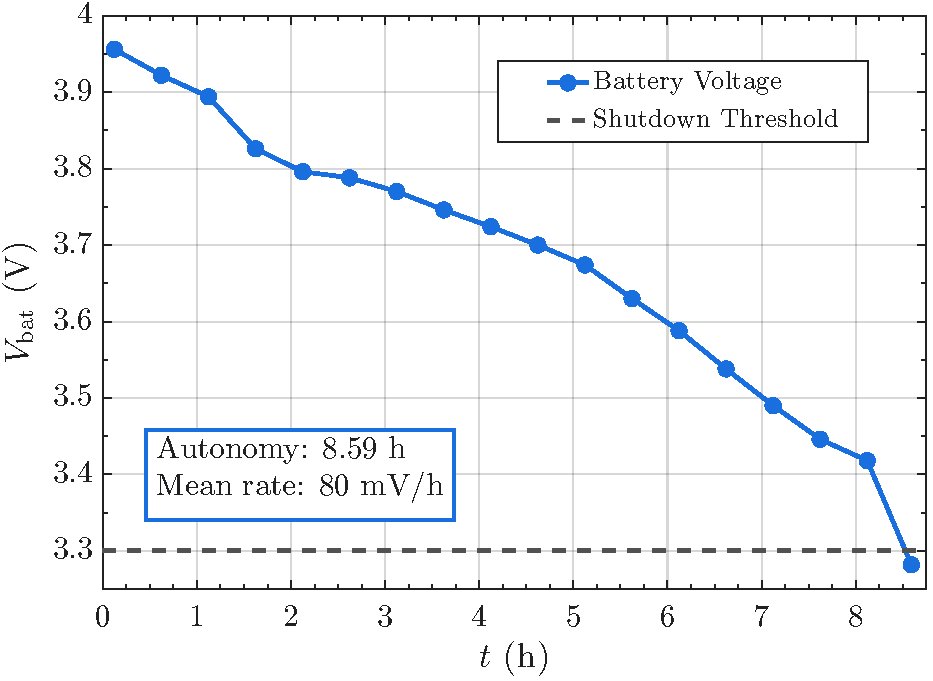
\includegraphics{images/battery.pdf}}
  \end{center}
  \smallcap{Continuous operation at 100 interrupts/second. DORI operated for approximately 8.6~hours before the 3.3~V cutoff, at a mean discharge rate of 80~mV/h.}
\end{frame}

% ======================================================================
\sectiondivider{Appendix}

% ---- tab:sources -----------------------------------------------------
\begin{frame}
  \frametitle{Sealed Source Activities}
  \begin{center}
  \renewcommand{\arraystretch}{1.4}
  \begin{tabular}{c c c c}
    \toprule
    \textbf{Source} & \textbf{Reference Activity} & \textbf{Reference Date} & \textbf{Serial Number} \\
    \midrule
    $^{241}$Am & TODO & TODO & TODO \\
    $^{109}$Cd & TODO & TODO & TODO \\
    $^{57}$Co  & TODO & TODO & TODO \\
    \bottomrule
  \end{tabular}
  \end{center}
  \smallcap{Reference activity of the sealed sources used throughout the hardware and calibration chapters. Values to be completed in the thesis.}
\end{frame}

% ---- fig:bc408 -----------------------------------------------------
\begin{frame}
  \frametitle{BC-408 Photon Absorption in 5 mm}
  \begin{center}
    \adjustbox{max width=0.7\textwidth,max height=0.72\textheight}{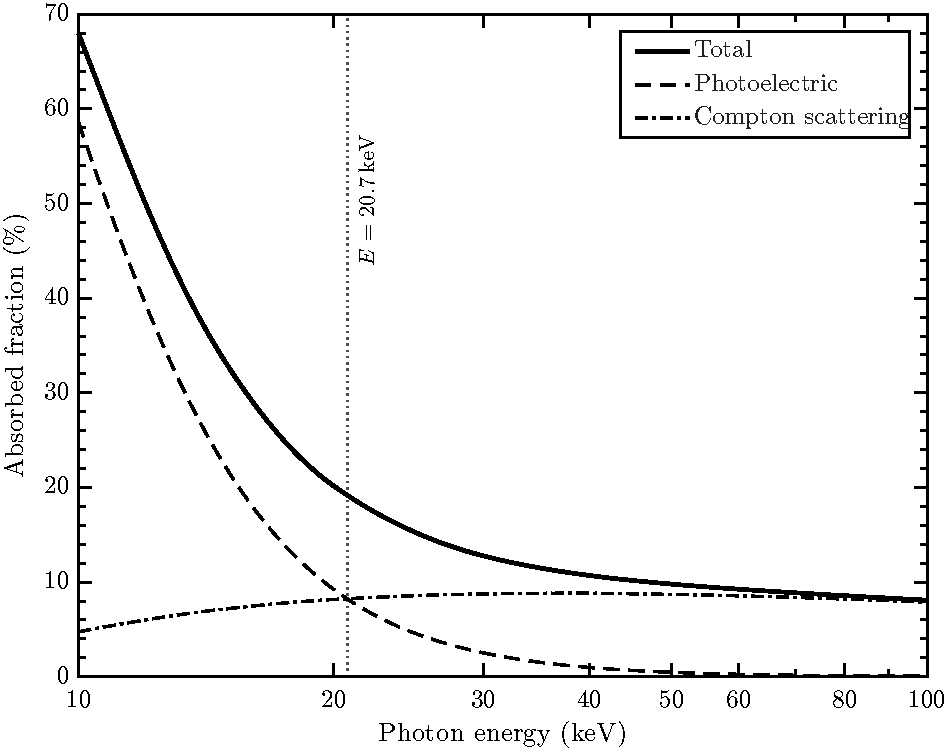
\includegraphics{images/bc408.pdf}}
  \end{center}
\end{frame}

% ======================================================================
\begin{frame}[plain]
  \centering
  \vfill
  {\Huge\bfseries\color{doriblue} Thank you}\\[0.5cm]
  {\large Marta Alexandra Moniz Rodrigues}
  \vfill
\end{frame}

\end{document}
